\documentclass[aspectratio=169, 9pt]{beamer}

\usepackage{makecell}
\usepackage{etoolbox}
\usepackage{biblatex}
\usepackage{tikz} % for graph
\usepackage{bbding}
\usepackage{layouts}
\usepackage{layout}
\newcommand\Wider[2][3em]{%
\makebox[\linewidth][c]{%
  \begin{minipage}{\dimexpr\textwidth+#1\relax}
  \raggedright#2
  \end{minipage}%
  }%
}
\usepackage{hyperref} % hyper text
\usepackage{booktabs} % To thicken table lines
\usepackage[normalem]{ulem} % for striking words

%margins
\newenvironment{changemargin}[2]{%
\begin{list}{}{%
\setlength{\topsep}{0pt}%
\setlength{\leftmargin}{#1}%
\setlength{\rightmargin}{#2}%
\setlength{\listparindent}{\parindent}%
\setlength{\itemindent}{\parindent}%
\setlength{\parsep}{\parskip}%
}%
\item[]}{\end{list}}

% code formating
\usepackage{xcolor}
\usepackage{listings} 
\lstset{basicstyle=\ttfamily,
  showstringspaces=false,
  commentstyle=\color{red},
  keywordstyle=\color{blue}
}
\definecolor{codegreen}{rgb}{0,0.6,0}
\definecolor{codegray}{rgb}{0.5,0.5,0.5}
\definecolor{codepurple}{rgb}{0.58,0,0.82}
\definecolor{backcolour}{rgb}{0.95,0.95,0.92}
\definecolor{bgturq}{RGB}{35,55,59}

\lstdefinestyle{mystyle}{
  backgroundcolor=\color{backcolour},   
  commentstyle=\color{codegreen},
  keywordstyle=\color{magenta},
  numberstyle=\tiny\color{codegray},
  stringstyle=\color{codepurple},
  basicstyle=\ttfamily\footnotesize,
  breakatwhitespace=false,         
  breaklines=true,                 
  captionpos=b,                    
  keepspaces=true,                 
  numbers=left,                    
  numbersep=5pt,                  
  showspaces=false,                
  showstringspaces=false,
  showtabs=false,                  
  tabsize=2
}

% ADD '-pdflua' as argument of latexmk
% Ref https://mirror.ibcp.fr/pub/CTAN/macros/luatex/latex/emoji/emoji-doc.pdf
\usepackage{emoji}
% For linux : https://github.com/samuelngs/apple-emoji-linux
\setemojifont{Apple Color Emoji}

\usepackage[sfdefault]{FiraSans}
\usetheme{metropolis}           % Use metropolis theme
\usetikzlibrary{positioning,shapes,arrows,calc,fit,backgrounds,shapes.multipart}

\tikzset{box/.style={draw, rectangle, rounded corners, thick, node distance=7em, text width=6em, text centered, minimum height=3.5em}}
\tikzset{line/.style={draw, thick, -latex'}}
\tikzset{every node/.style={font=\scriptsize}}

% Graphics and Videos
% https://tex.stackexchange.com/questions/89088/how-to-embed-video-and-animation-in-latex-and-latex-beamer-step-by-step
\usepackage{graphicx} %The mode "LaTeX => PDF" allows the following formats: .jpg  .png  .pdf  .mps
\usepackage{animate}


%\usepackage[utf8]{inputenc}
%\usetheme{Antibes}
\usefonttheme{professionalfonts}

\setbeamertemplate{itemize items}[circle]

%\bibliography{presentation}

\newcommand\blfootnote[1]{%
  \begingroup
  \renewcommand\thefootnote{}\footnote{{\tiny #1}}%
  \addtocounter{footnote}{-1}%
  \endgroup
}

\usepackage{csvsimple}

%%%%%%%%%%%%%%%%%%%%%%%%%%%%%%%%%%%%%%%%%%%%%%%%%%%%%%%%%%%%%%%%%%%%%%%%%%%%%%%%%%%%%
%Page de titre %%%%%%%%%%%%%%%%%%%%%%%%%%%%%%%%%%%%%%%%%%%%%%%%%%%%%%%%%%%%%%%%%%%%%%
%%%%%%%%%%%%%%%%%%%%%%%%%%%%%%%%%%%%%%%%%%%%%%%%%%%%%%%%%%%%%%%%%%%%%%%%%%%%%%%%%%%%%
\title[\emoji{dna} Analyse Exome CLOVES ]{\emoji{dna} Analyse Exomes CLOVES }

\author{Dr. Thomas Steimlé}
\institute[OH]{
  Laboratoire d'oncohématologie de l'hôpital Necker \\
  \vfill
  \begin{figure}[!b]
    \centering

    
\includegraphics[height=1cm]{Images/1200aphp.pdf}\hspace*{5.5cm}~
    
\includegraphics[height=1.5cm]{Images/necker.pdf}
  \end{figure}
}
\date{Mars 2023}

\begin{document}

\begin{frame}
    \maketitle
    \thispagestyle{empty}
\end{frame}

\section{Materials \& Methods}

\begin{frame}
    \frametitle{\emoji{busts-in-silhouette} Matériel, N = 24 paires N/P}
    \begin{center}
        {\scriptsize
            \csvreader[
                tabular = lccc,
                table head = \toprule \textbf{Alias} & \textbf{Cases} & \textbf{Patho} & \textbf{Normal} \\\midrule,
                table foot = \bottomrule
                ]{data/samples.csv}%
                {alias=\alias, Nom=\nom, Prenom=\prenom, Patho=\patho, Normal=\normal}{%
                \alias & \nom~\prenom & \patho & \normal
            }
        }
    \end{center}
\end{frame}

\begin{frame}
    \frametitle{\emoji{straight-ruler} Méthodes}
    \begin{itemize}
      \item[] \emoji{dna} Séquençage selon la méthode \textit{Agilent SureSelect Human All Exon V7 panel} sur automates \textit{Illumina Next/NovaSeq}.
      \vskip 0.2in
      \item[] \emoji{floppy-disk} Analyse bioinformatique:
      \vskip 0.1in
      \quad Alignement (hg19 bwa mem v0.7.17-r1188) et déduplication UMI (umi\_tools v1.1.1)
      \vskip 0.1in
      \quad Callers : 
      \vskip 0.05in
      \begin{itemize}
        \item[\emoji{gear}] \quad \textbf{mutect2} (GATK v4.2)
        \item[\emoji{gear}] \quad \textbf{strelka} (Illumina v2.9.10)
        \item[\emoji{gear}] \quad \textbf{lancet} (NY Genome Center v1.1.0)
      \end{itemize}
      \vskip 0.05in
      \item[] \quad En suivant les modes opératoires displonibles (cf. diapos supplémentaires).
    \end{itemize}
\end{frame}

\section{Results}

\begin{frame}[t]
    \frametitle{\emoji{left-right-arrow} Alignment -- proportions of targeted sequences at given depth by case}
    \begin{columns}[T]
        \begin{column}{.5\textwidth}
            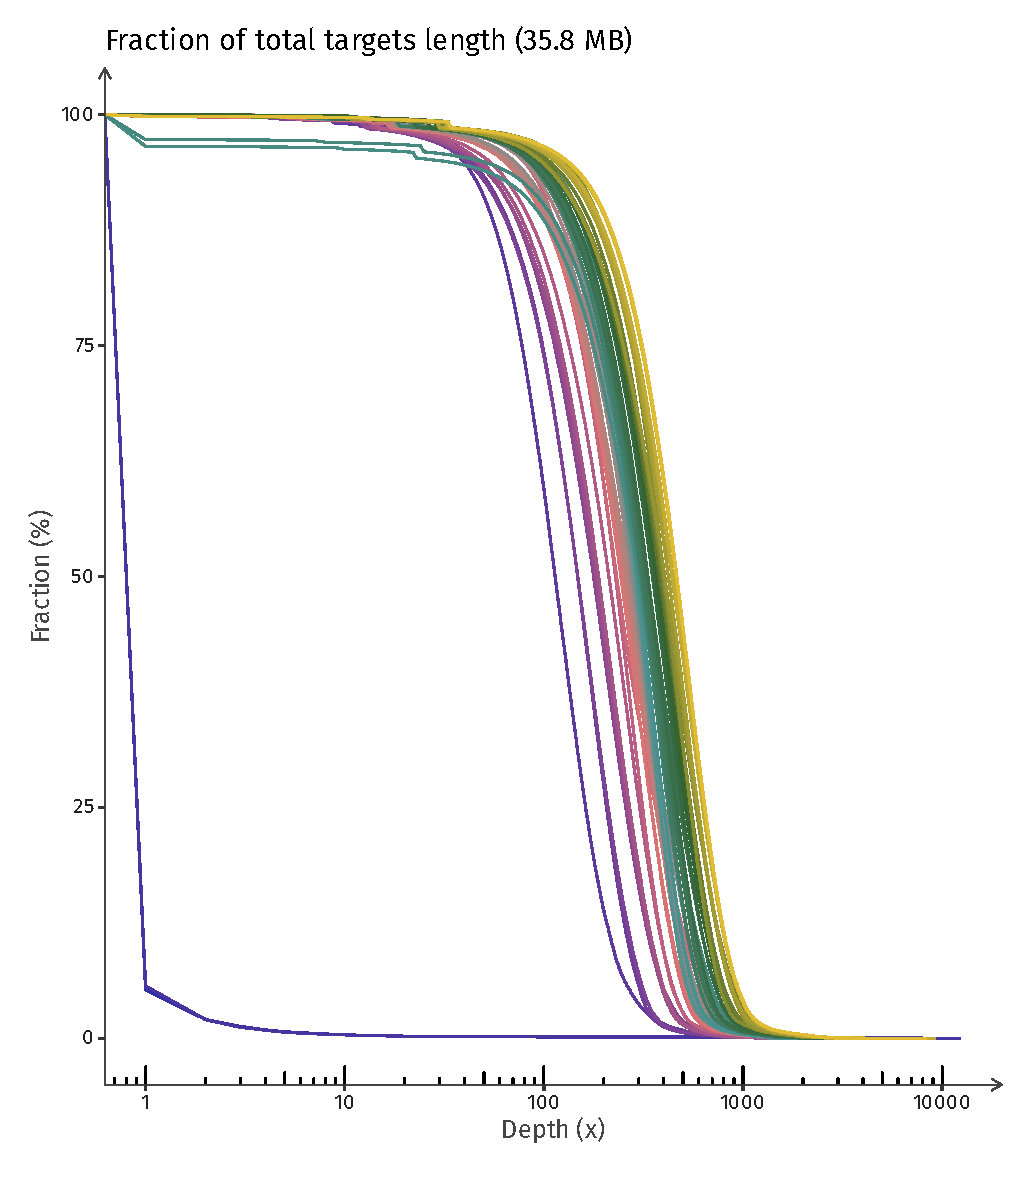
\includegraphics[height=.95\textheight]{Images/coverages.pdf}
        \end{column}
        \begin{column}{.25\textwidth}
            {\scriptsize
                \csvreader[
                    tabular = llr,
                    table head = \toprule  & \textbf{Case} & \textbf{$<$ 100x (\%)} \\\midrule,
                    ]{data/cov50_head.csv}%
                    {sample=\sample,cov=\cov,fra=\fra,col=\col}{%
                    {\color[HTML]{\col} \textbf{---}} & \sample & \fra 
                }
            }
        \end{column}
        \begin{column}{.25\textwidth}
            {\scriptsize
                \csvreader[
                    tabular = llr,
                    table head = \\ \\,
                    table foot = \bottomrule
                    ]{data/cov50_tail.csv}%
                    {sample=\sample,cov=\cov,fra=\fra,col=\col}{%
                    {\color[HTML]{\col} \textbf{---}} & \sample & \fra 
                }
            }
        \end{column}
    \end{columns}
\end{frame}

\begin{frame}
    \frametitle{\emoji{round-pushpin} Variant calling}
    \begin{figure}
        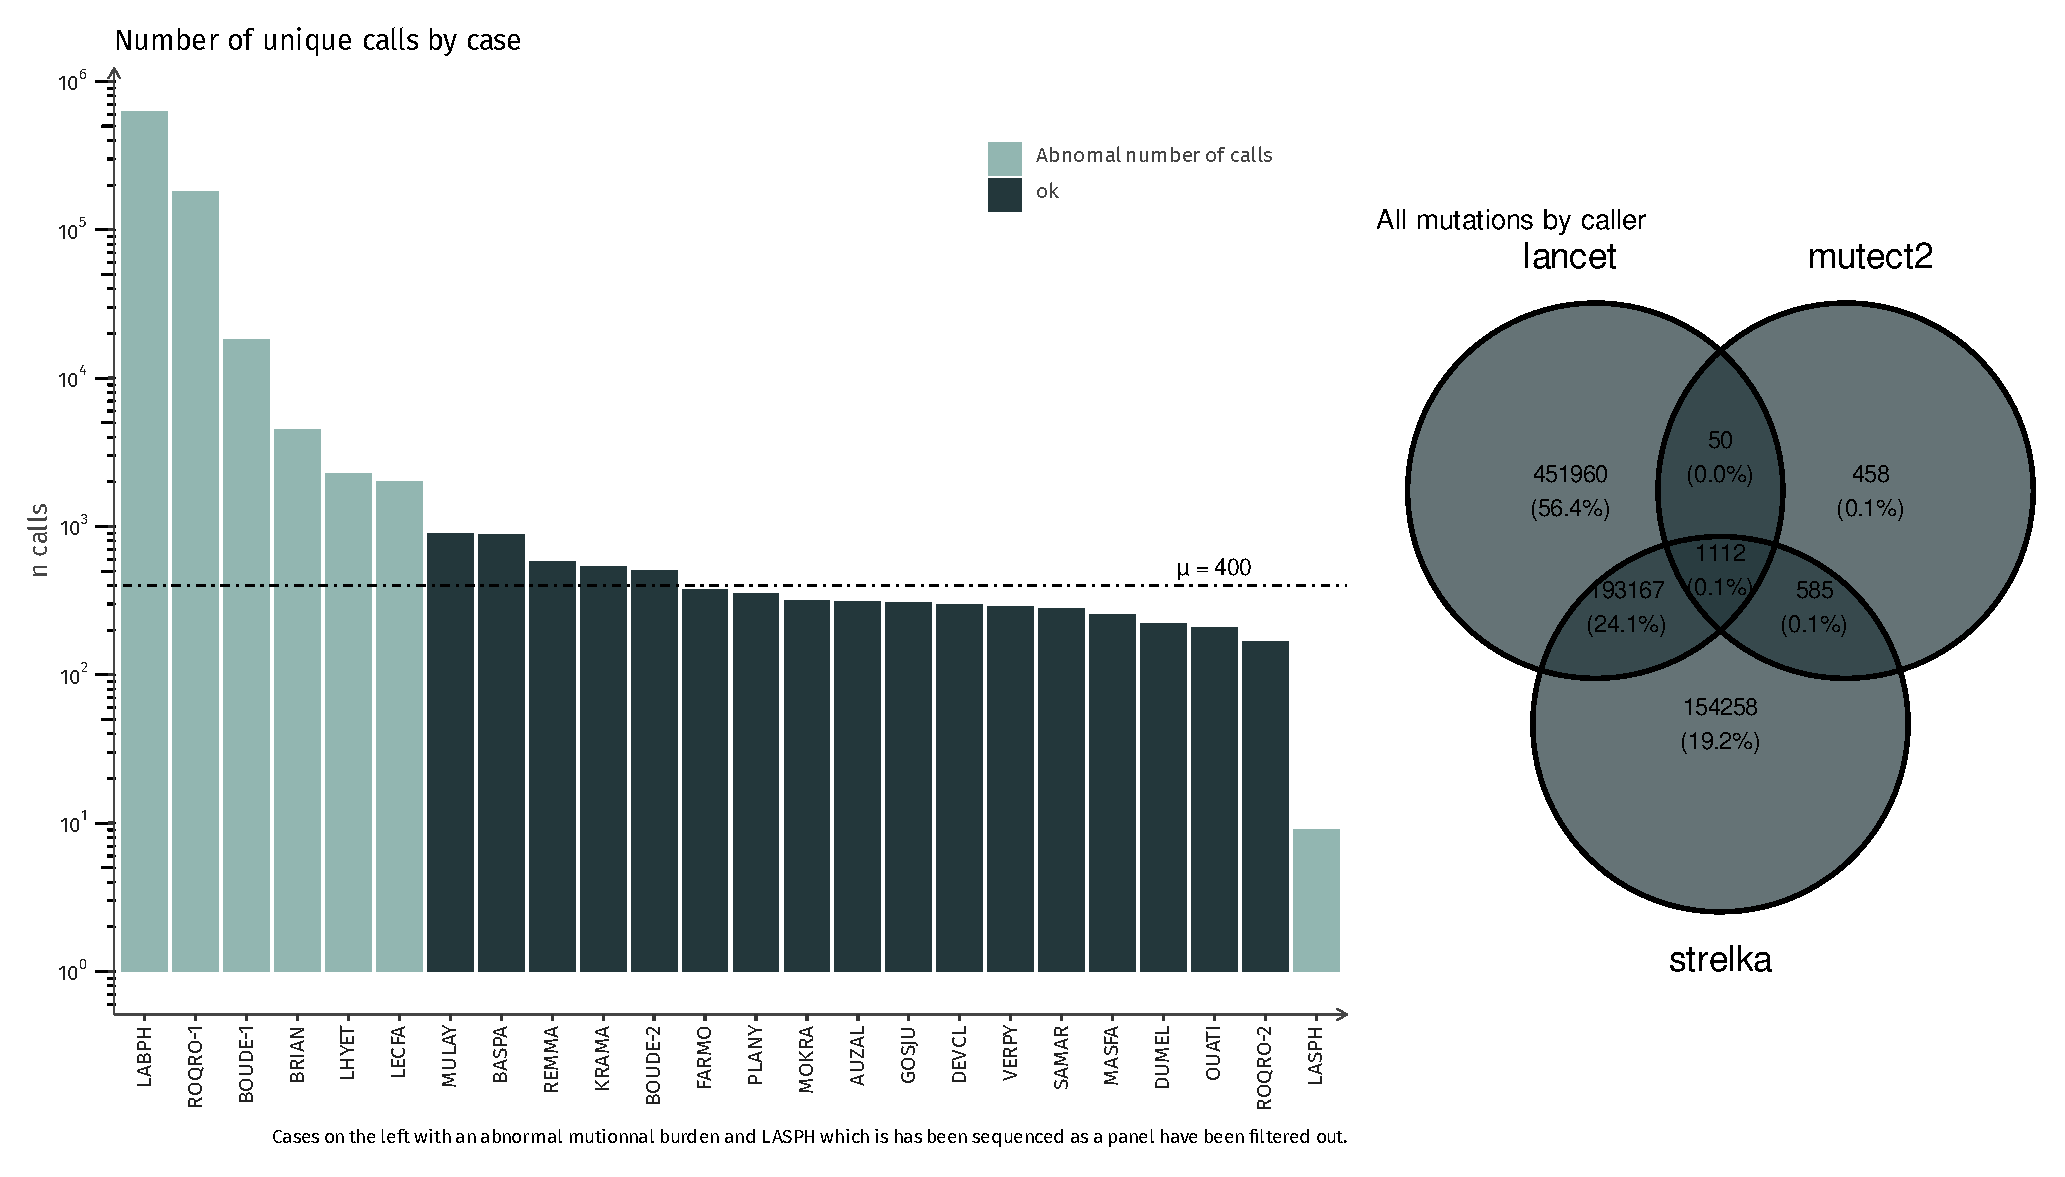
\includegraphics[height=.95\textheight]{Images/calls.pdf}
    \end{figure}
\end{frame}

\begin{frame} 
    \frametitle{\emoji{wastebasket} Filtering -- Proportion of filtered calls for each case}
    \begin{figure}
        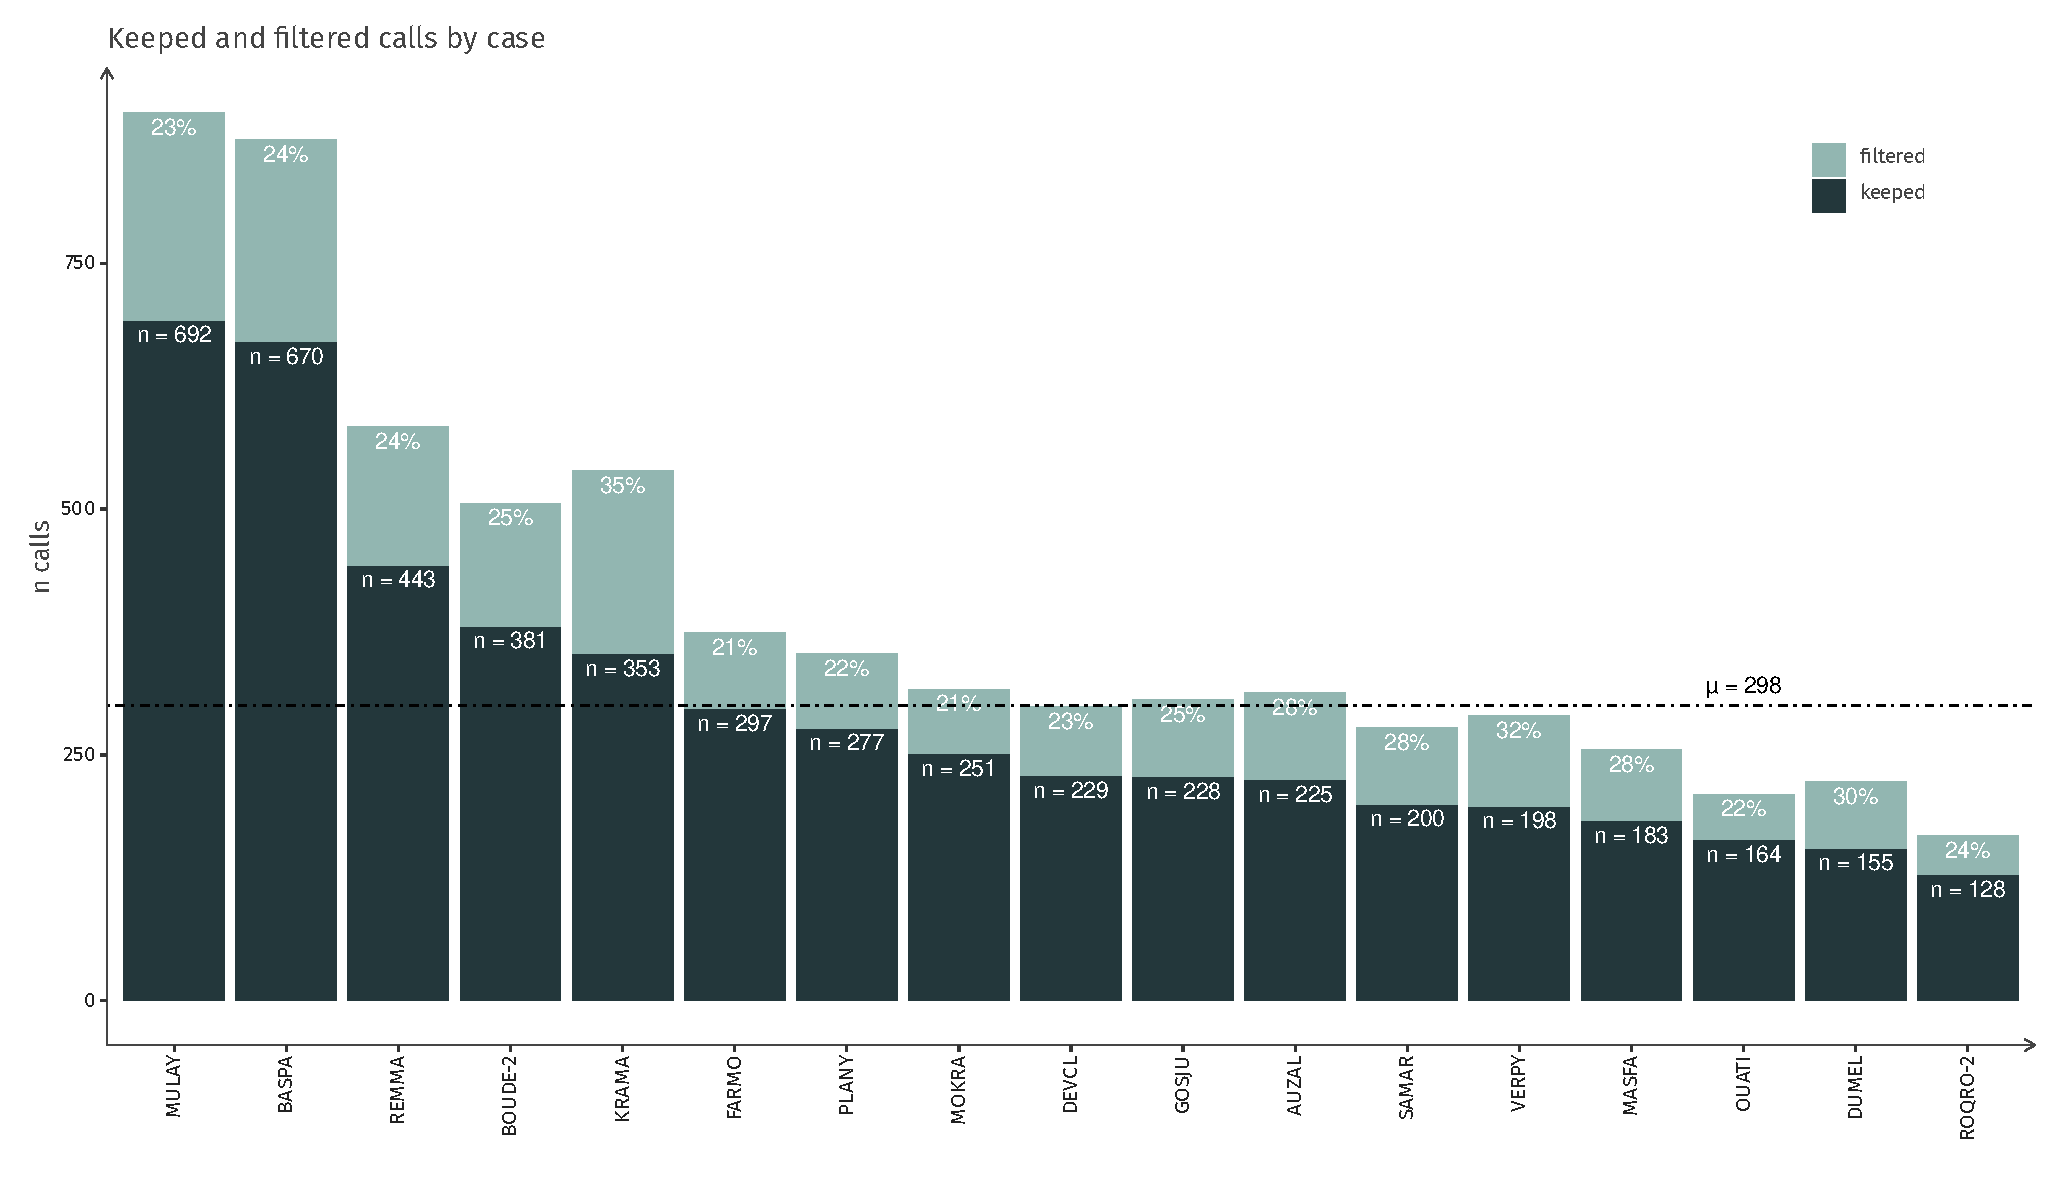
\includegraphics[height=.95\textheight]{Images/filter.pdf}
    \end{figure}
\end{frame}

\begin{frame}
    \frametitle{\emoji{wastebasket} Filtering -- Rules and resulting allelic fraction distribution}
    \begin{figure}
        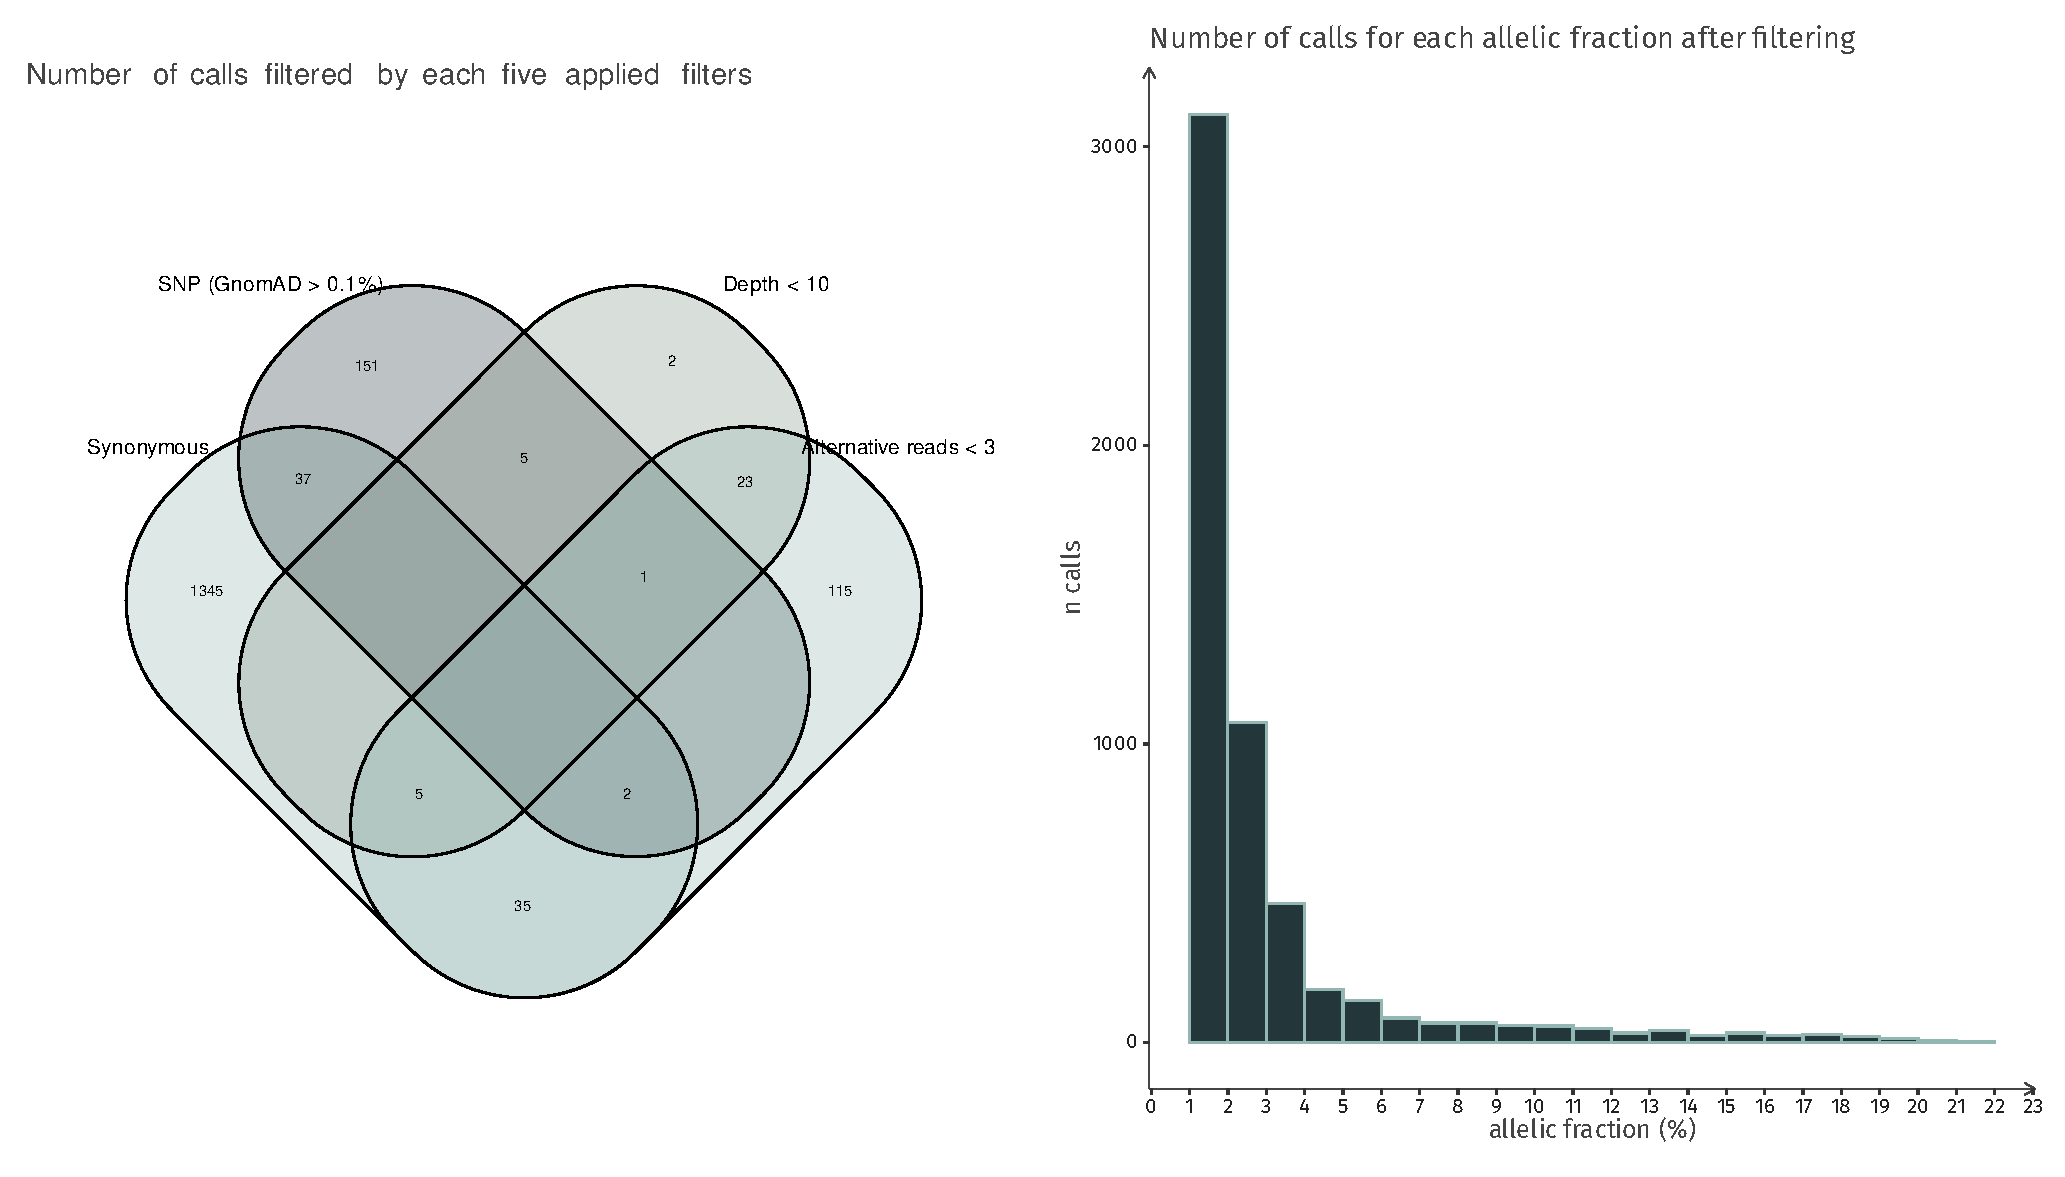
\includegraphics[height=.95\textheight]{Images/filter2.pdf}
    \end{figure}
\end{frame}

\begin{frame}
    \frametitle{\emoji{memo} Results -- Recurrent genes known as tumor suppressors or proto-oncogenes.}
    \begin{center}
        {\scriptsize
            \csvreader[
                tabular = lccr,
                table head = \toprule \textbf{Alias} & \textbf{Gene} & \textbf{Variant} & \textbf{VAF} (\%)\\\midrule,
                table foot = \bottomrule
                ]{data/recurrent_genes_cancer.csv}%
                {alias=\alias, Gene=\gene, VAR_p=\var, VAF=\vaf}{%
                \alias & \textit{\gene} & \var & \vaf
            }
        }
    \end{center}
\end{frame}

\begin{frame}
    \frametitle{\emoji{bar-chart} Results -- Over-representation analysis -- GoTerms}
    \begin{figure}
        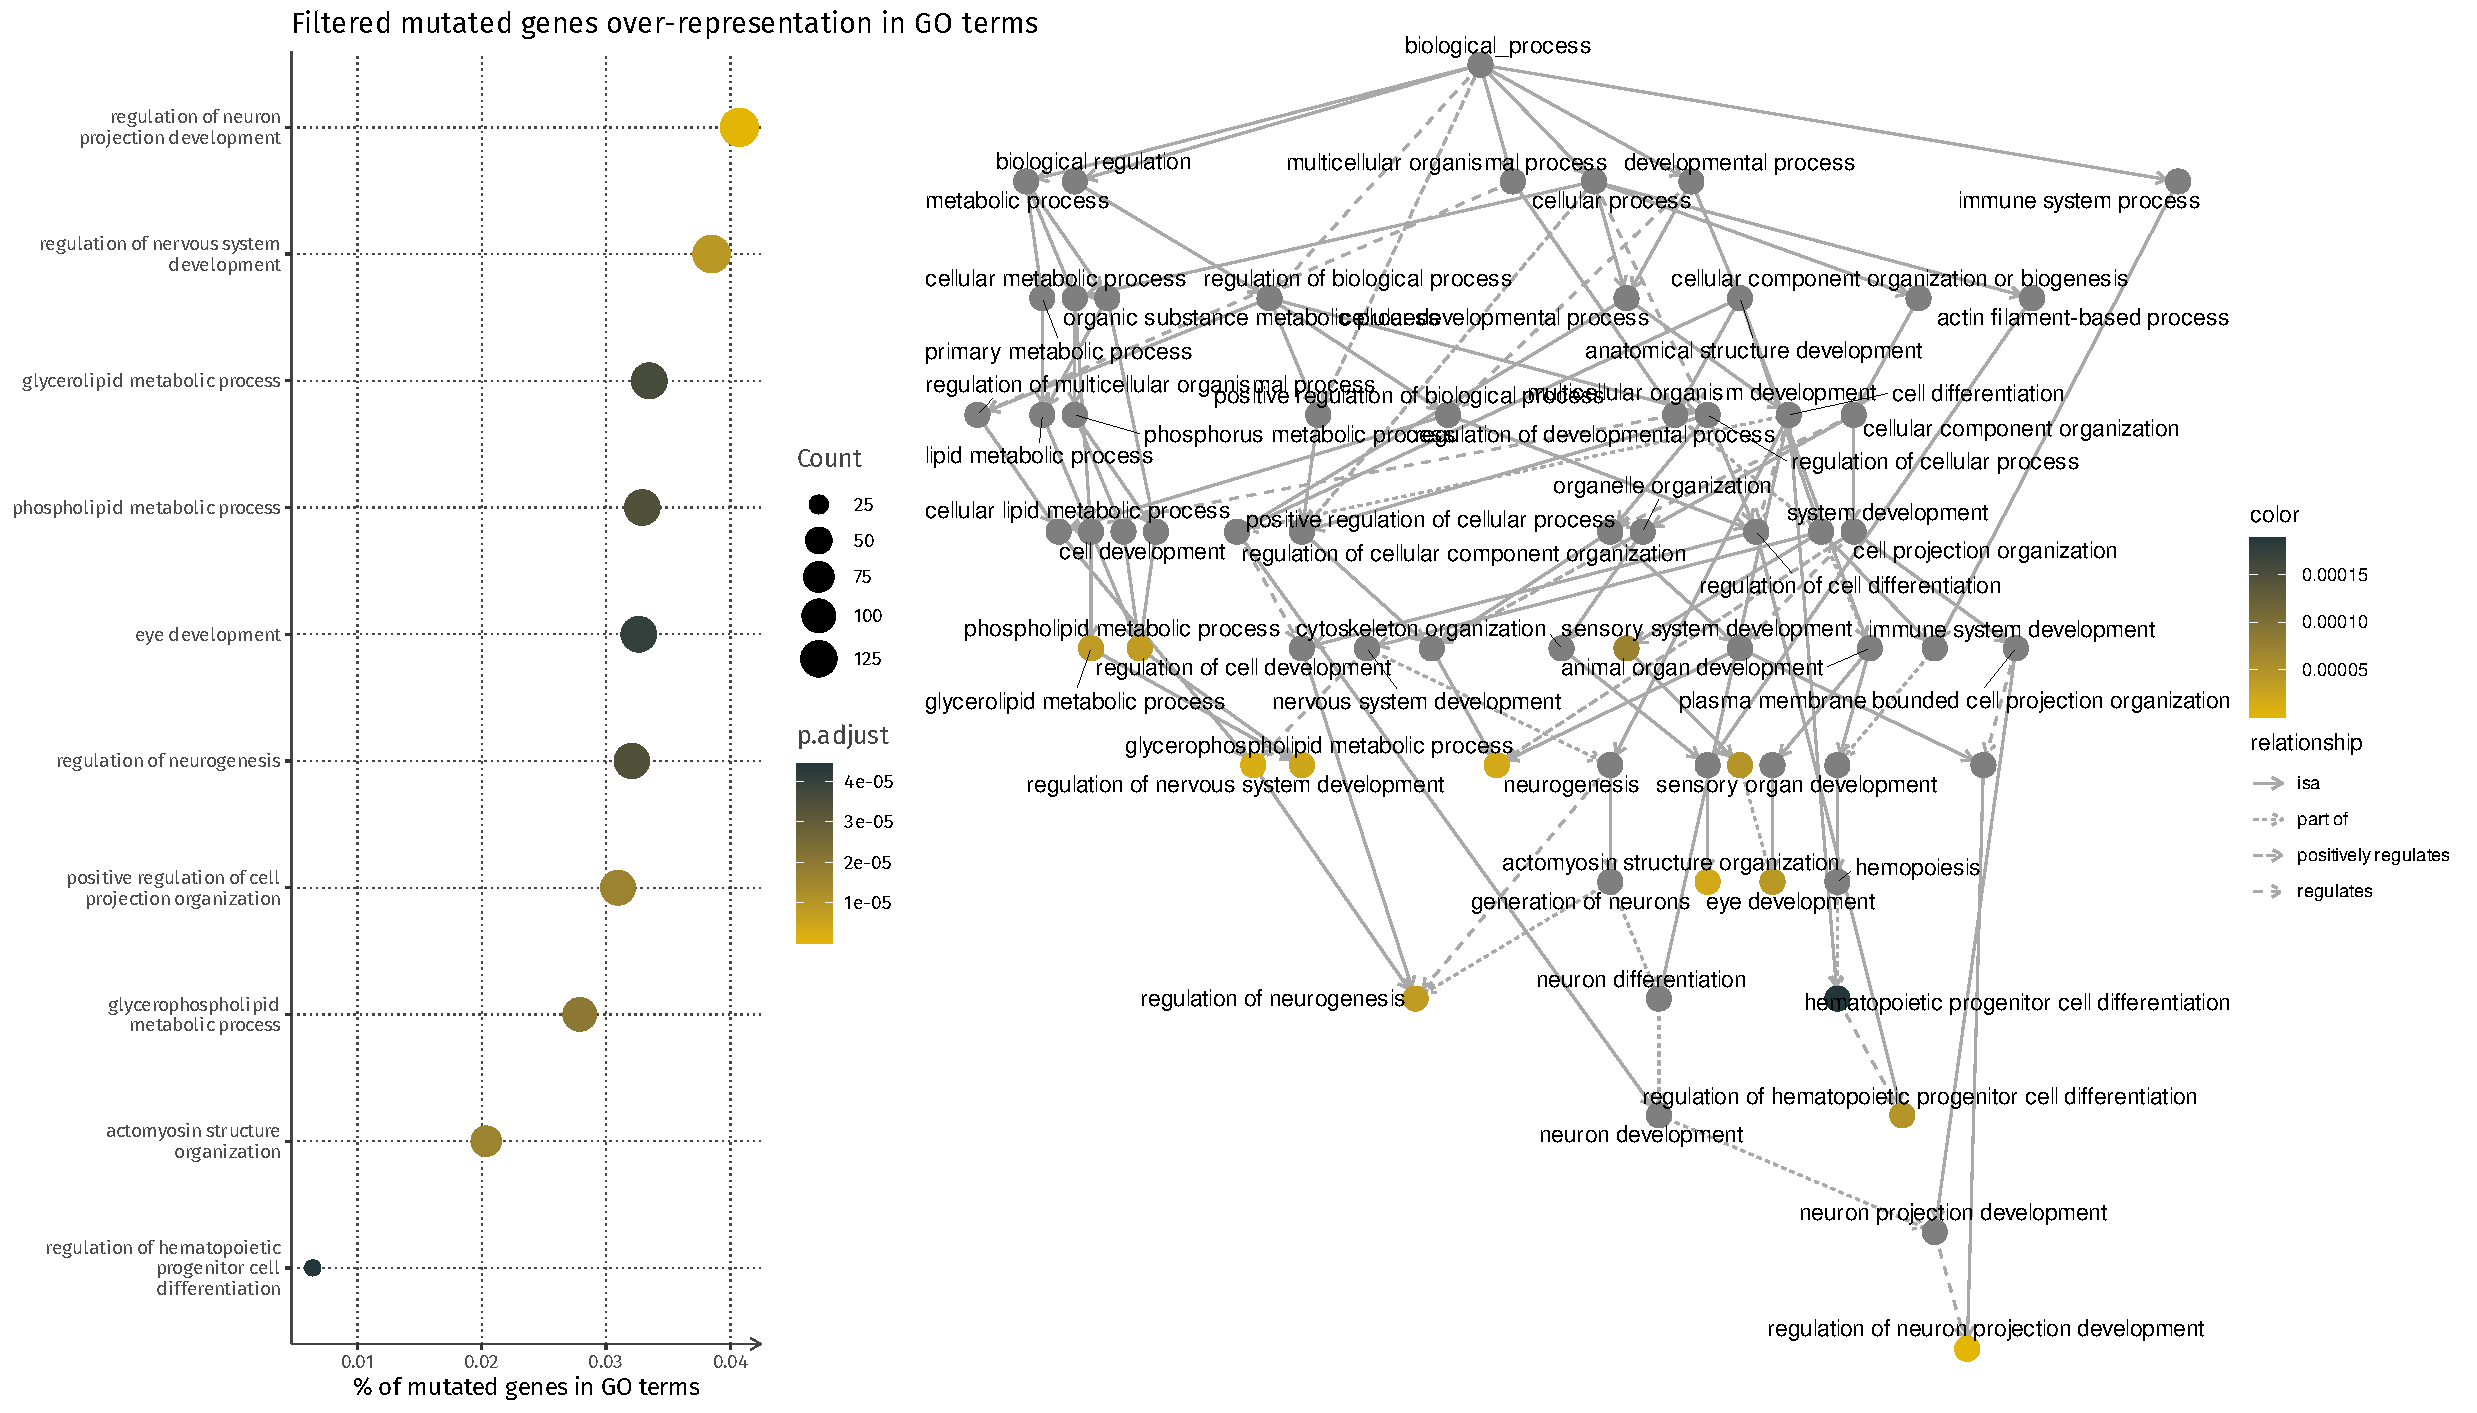
\includegraphics[width=.95\textwidth]{Images/enrich_go.pdf}
    \end{figure}
\end{frame}

\begin{frame}
    \frametitle{\emoji{bar-chart} Results -- Over-representation analysis -- KEGG pathways | WikiPathways | Reactome}
    \begin{figure}
        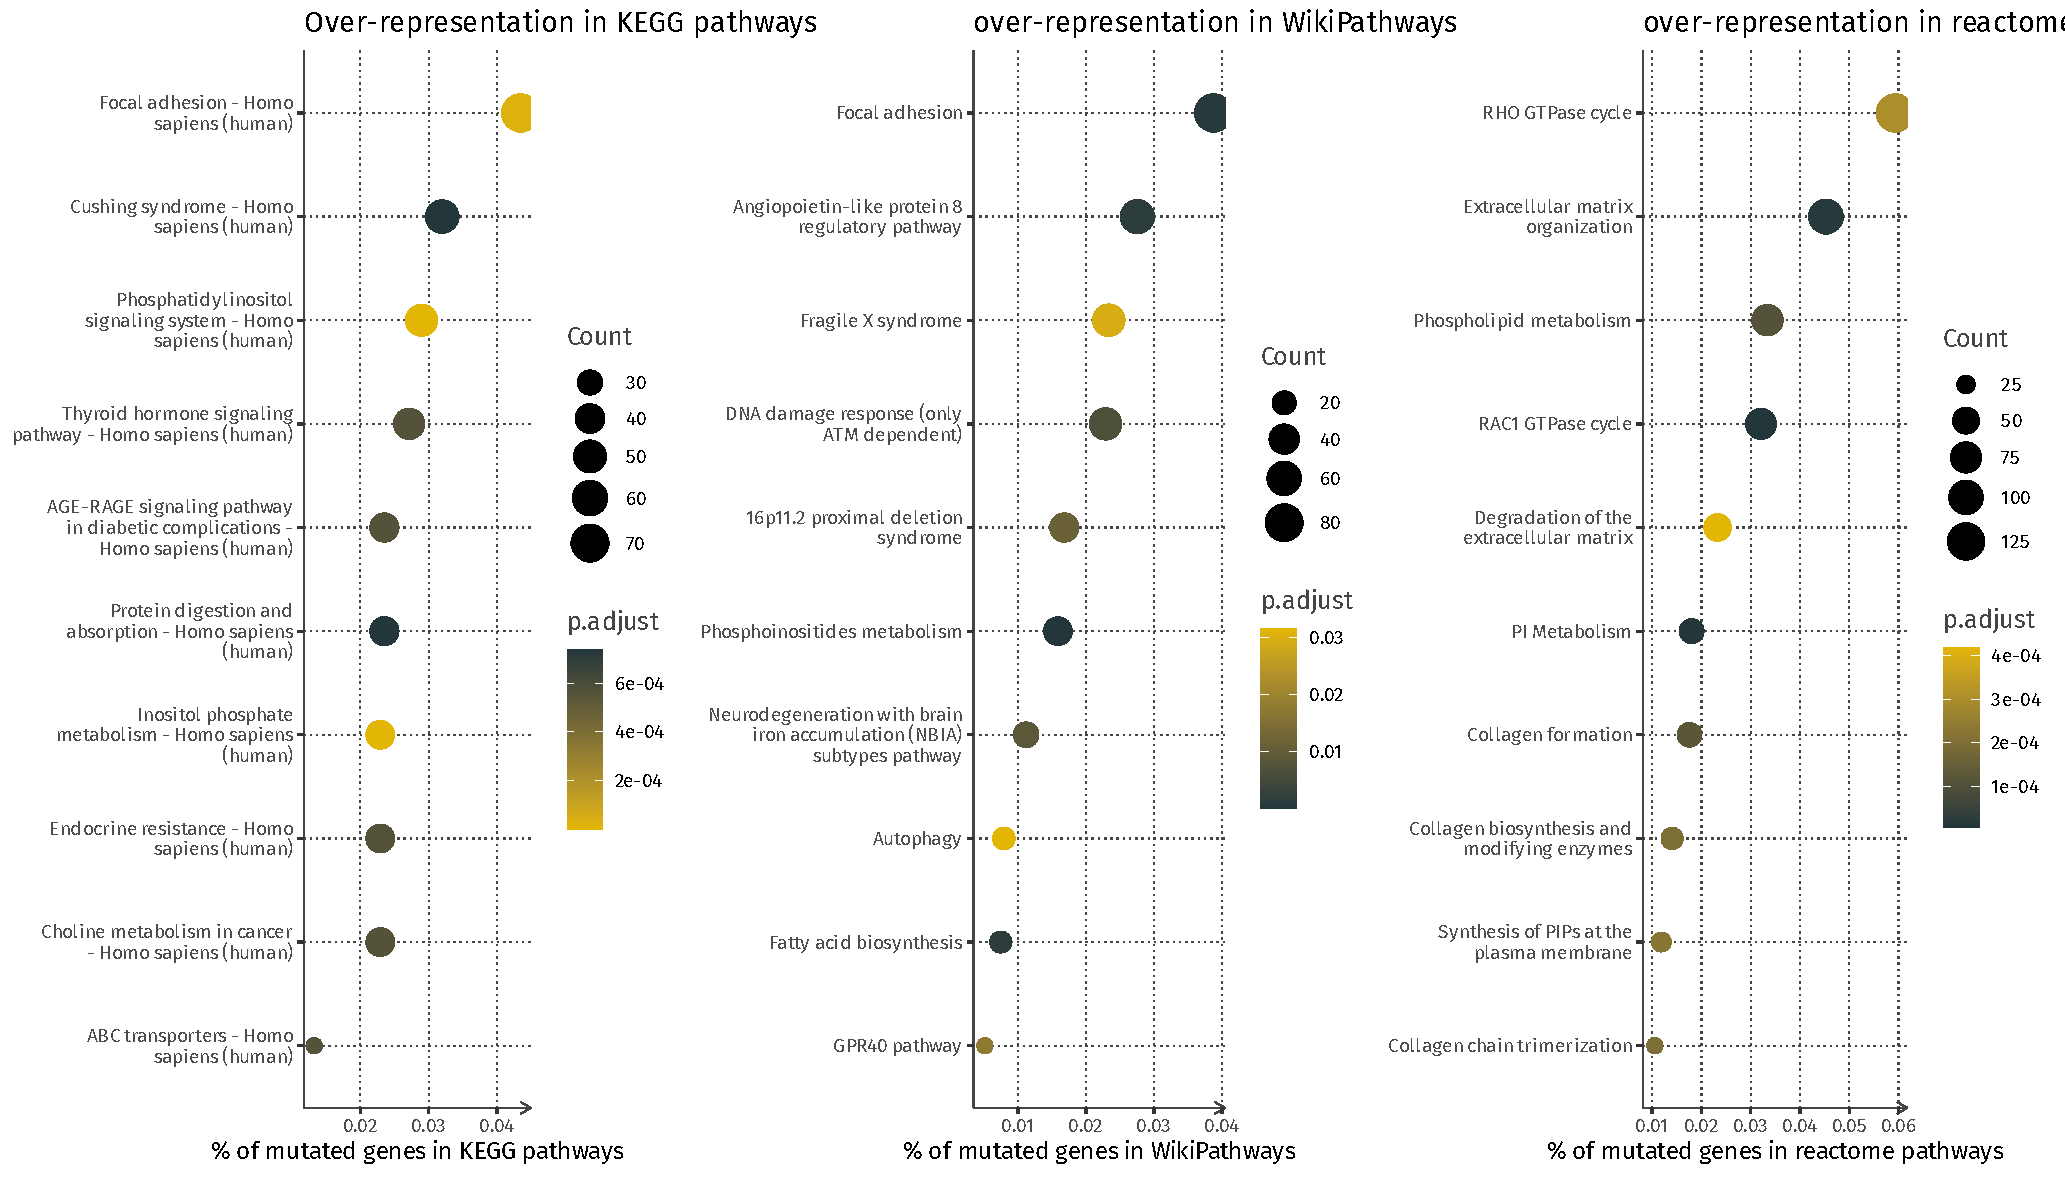
\includegraphics[width=.95\textwidth]{Images/enrich.pdf}
    \end{figure}
\end{frame}

\begin{frame}
    \frametitle{\emoji{compass} Results -- Over-representation analysis -- KEGG -- Phosphatidylinositol signaling system}
    \begin{columns}[T]
        \begin{column}{.75\textwidth}
            \begin{figure}
                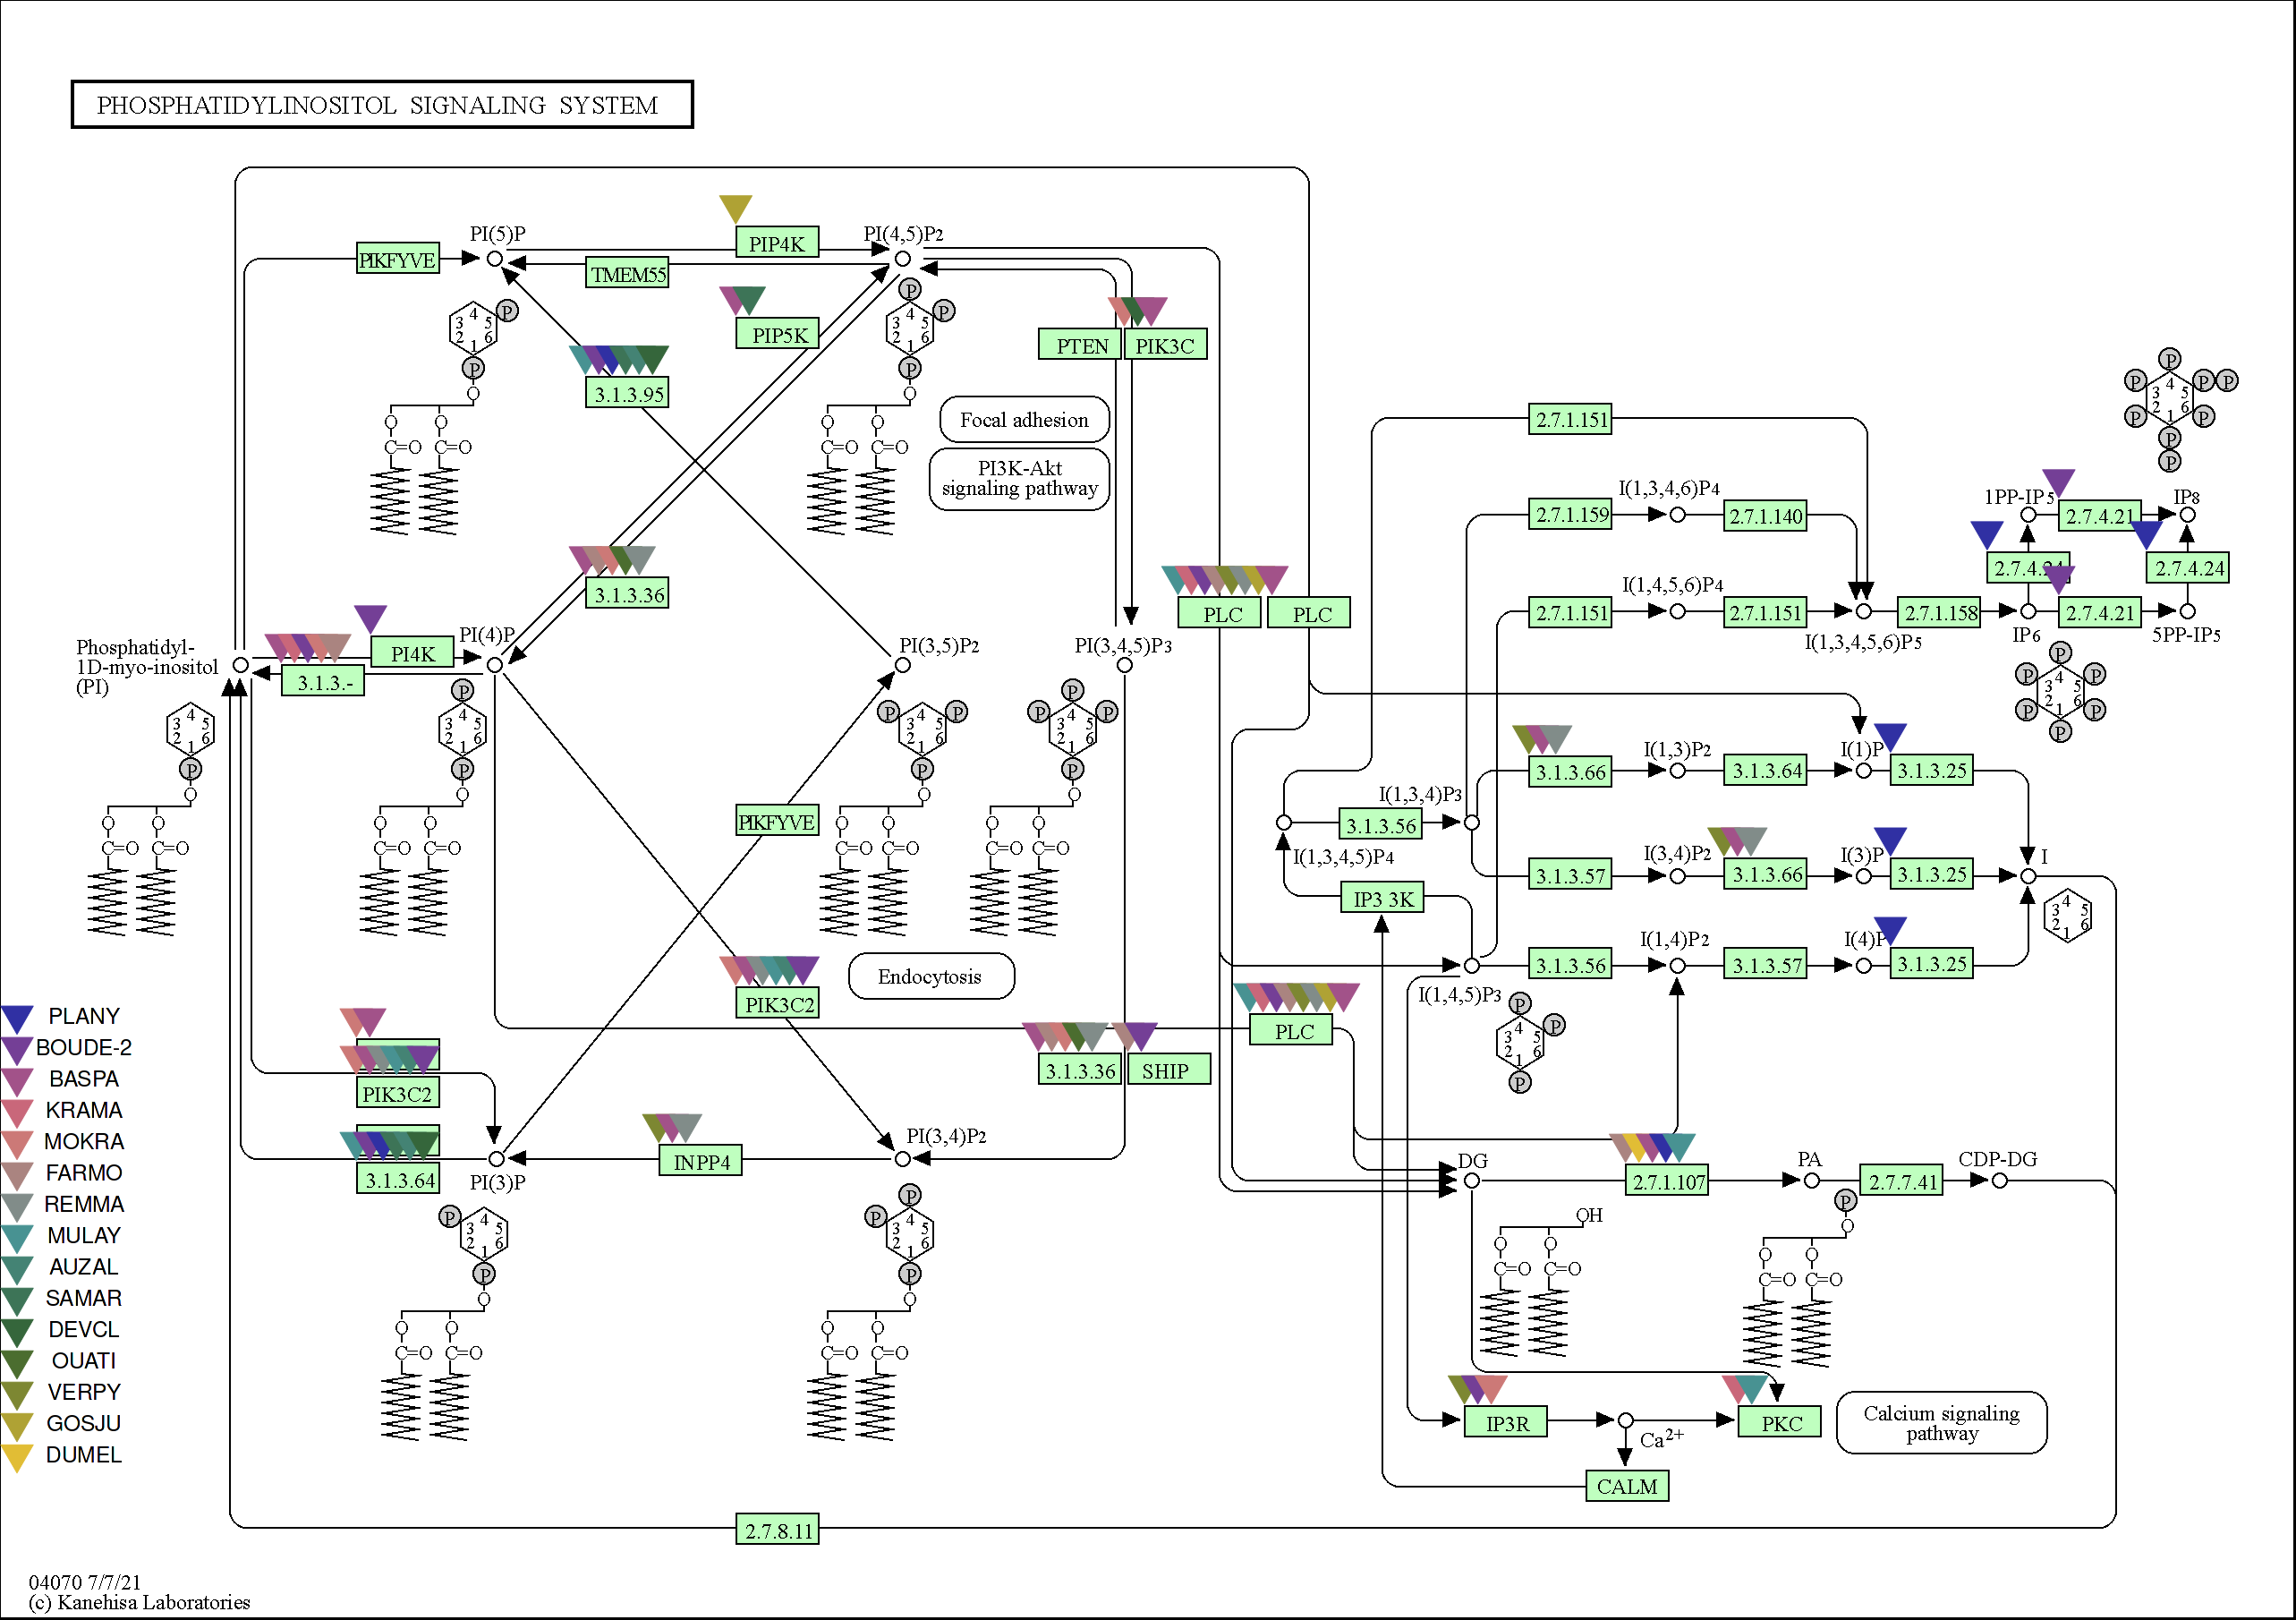
\includegraphics[height=.95\textheight]{Images/hsa04070.png}
            \end{figure}
        \end{column}
        \begin{column}{.25\textwidth}
            {\fontsize{3pt}{3.6pt}\selectfont
                \csvreader[
                    tabular = ll,
                    separator = tab,
                    table head = \textbf{Complexes:}\\,
                ]{data/hsa04070.tsv}%
                {ec=\ec,n=\num,name=\name}
                {\ec \\ \name}
            }
        \end{column}
    \end{columns}
\end{frame}

\begin{frame}
    \frametitle{\emoji{compass} Results -- Over-representation analysis -- KEGG -- Focal Adhesion}
    \begin{figure}
        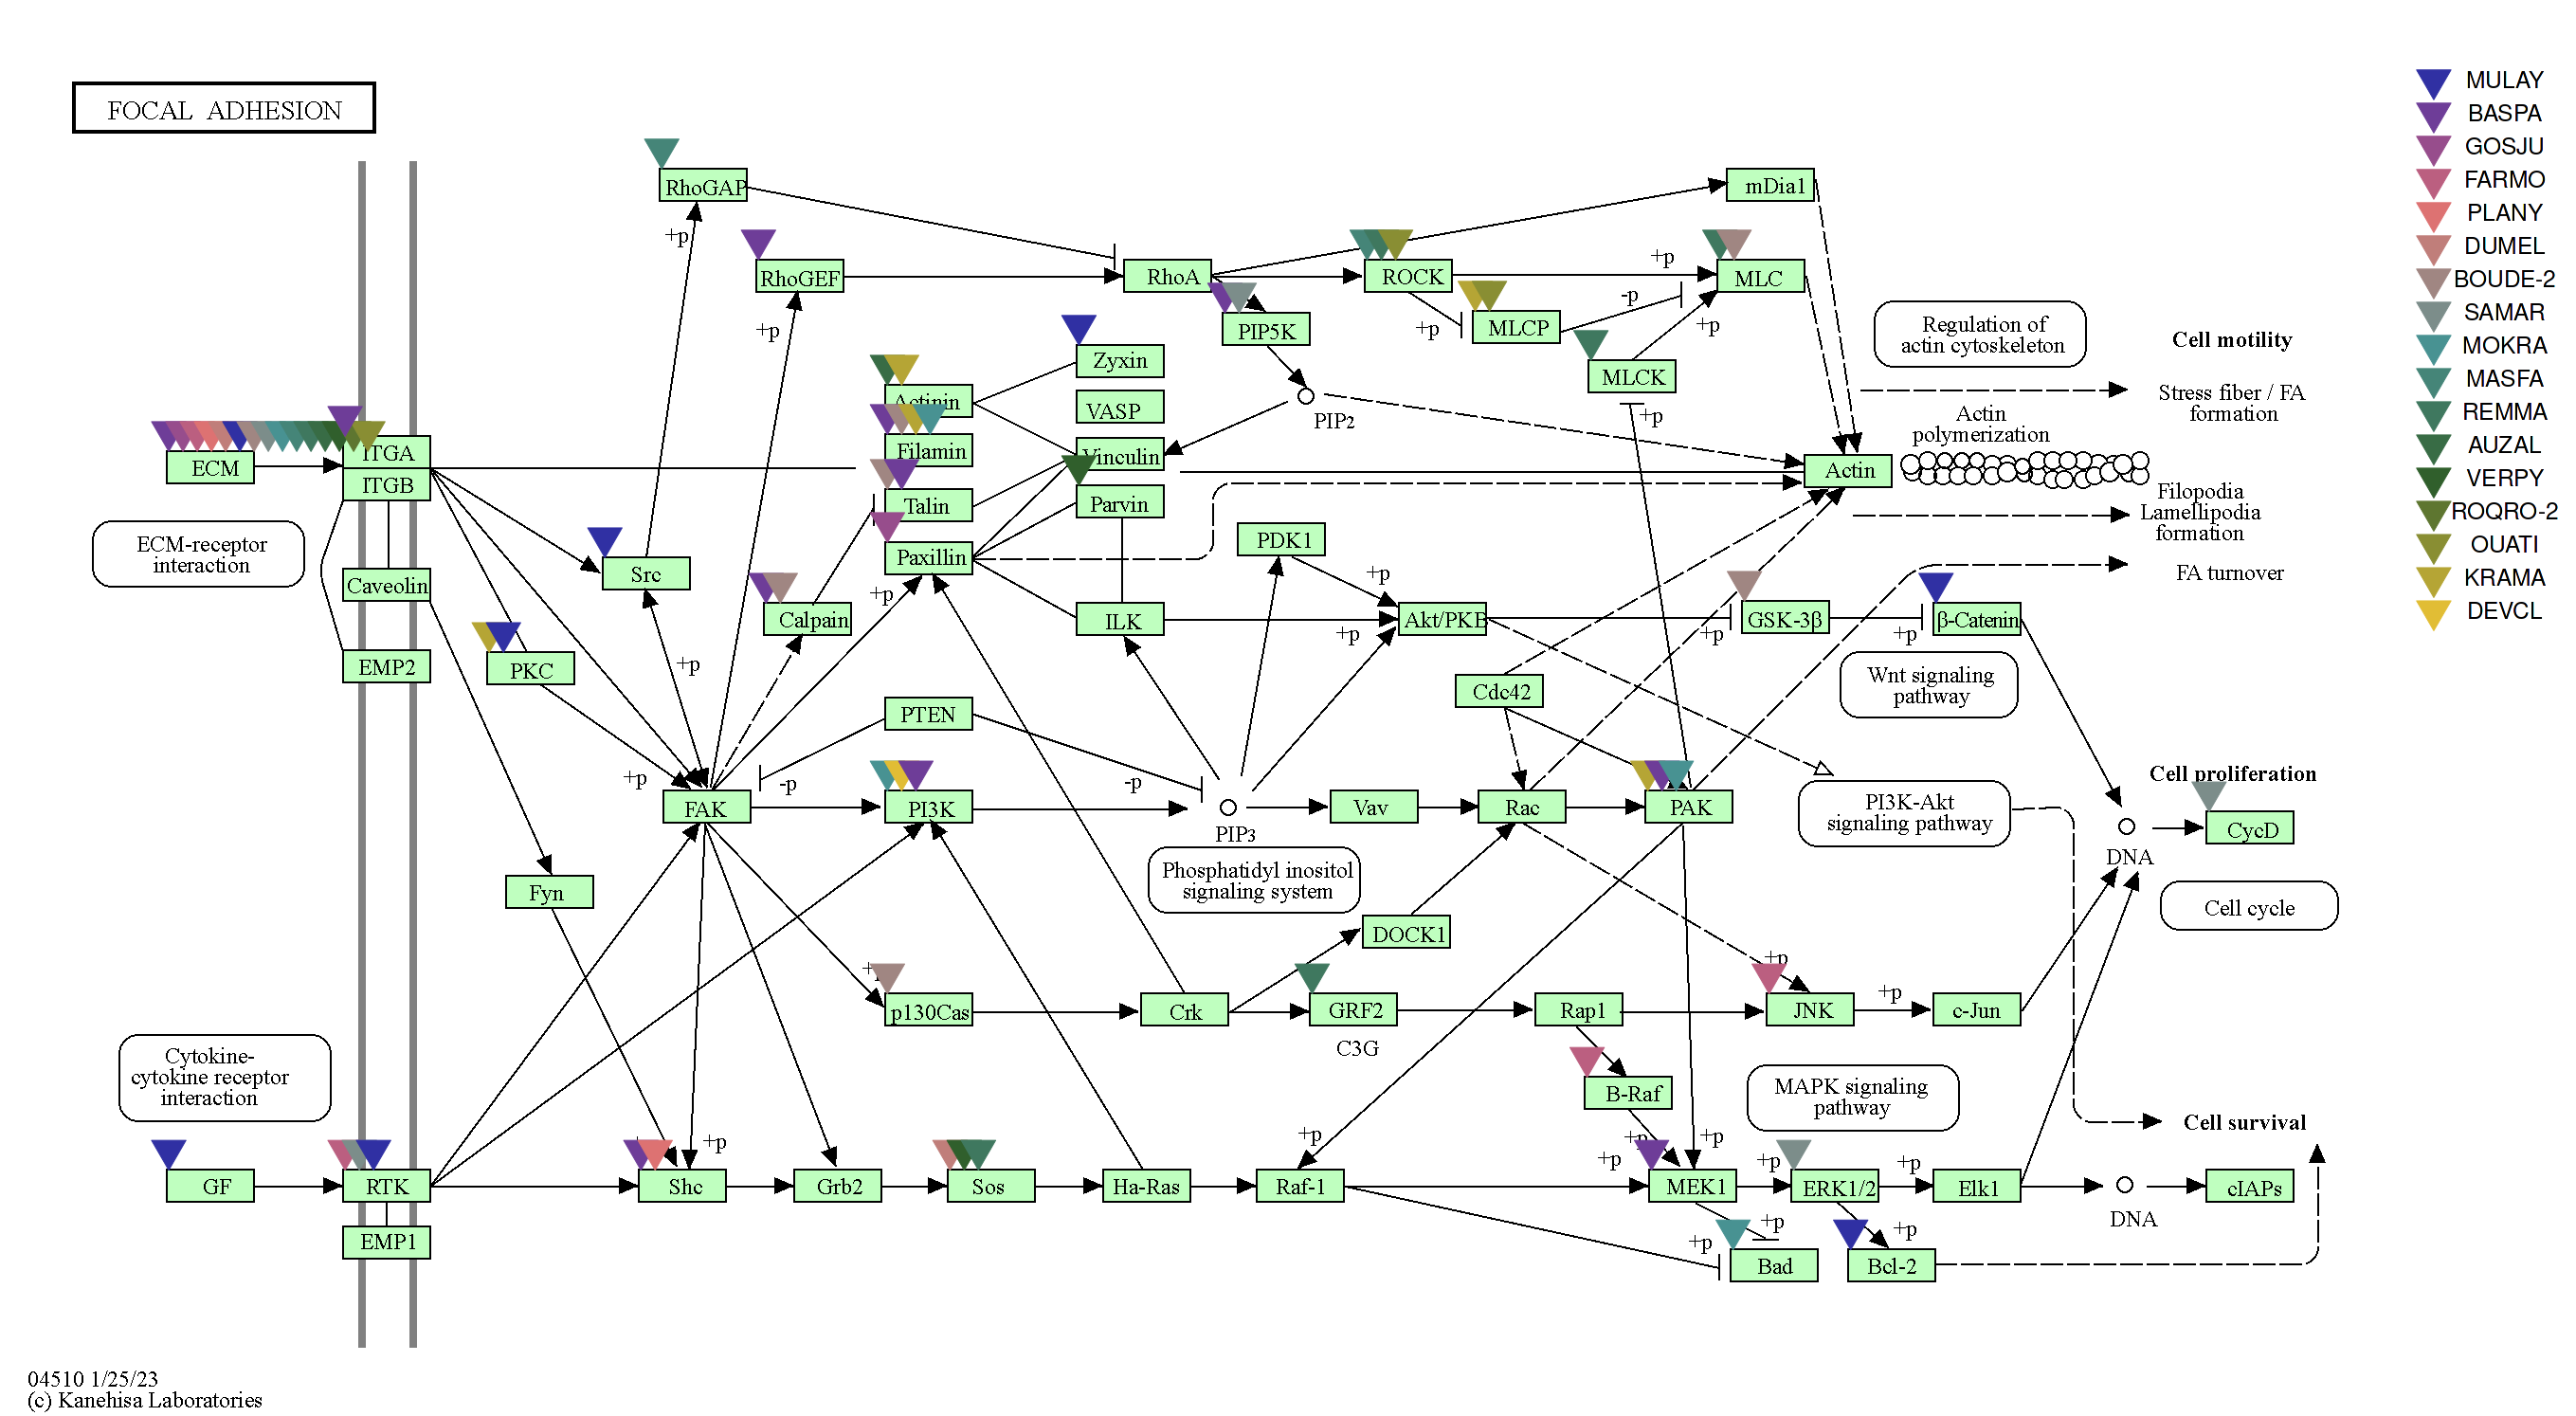
\includegraphics[width=.95\textwidth]{Images/hsa04510.png}
    \end{figure}
\end{frame}

\begin{frame}
    \frametitle{\emoji{compass} Results -- Over-representation analysis -- KEGG -- Inositol Phosphate Metabolism}
    \begin{columns}[T]
        \begin{column}{.75\textwidth}
            \begin{figure}
                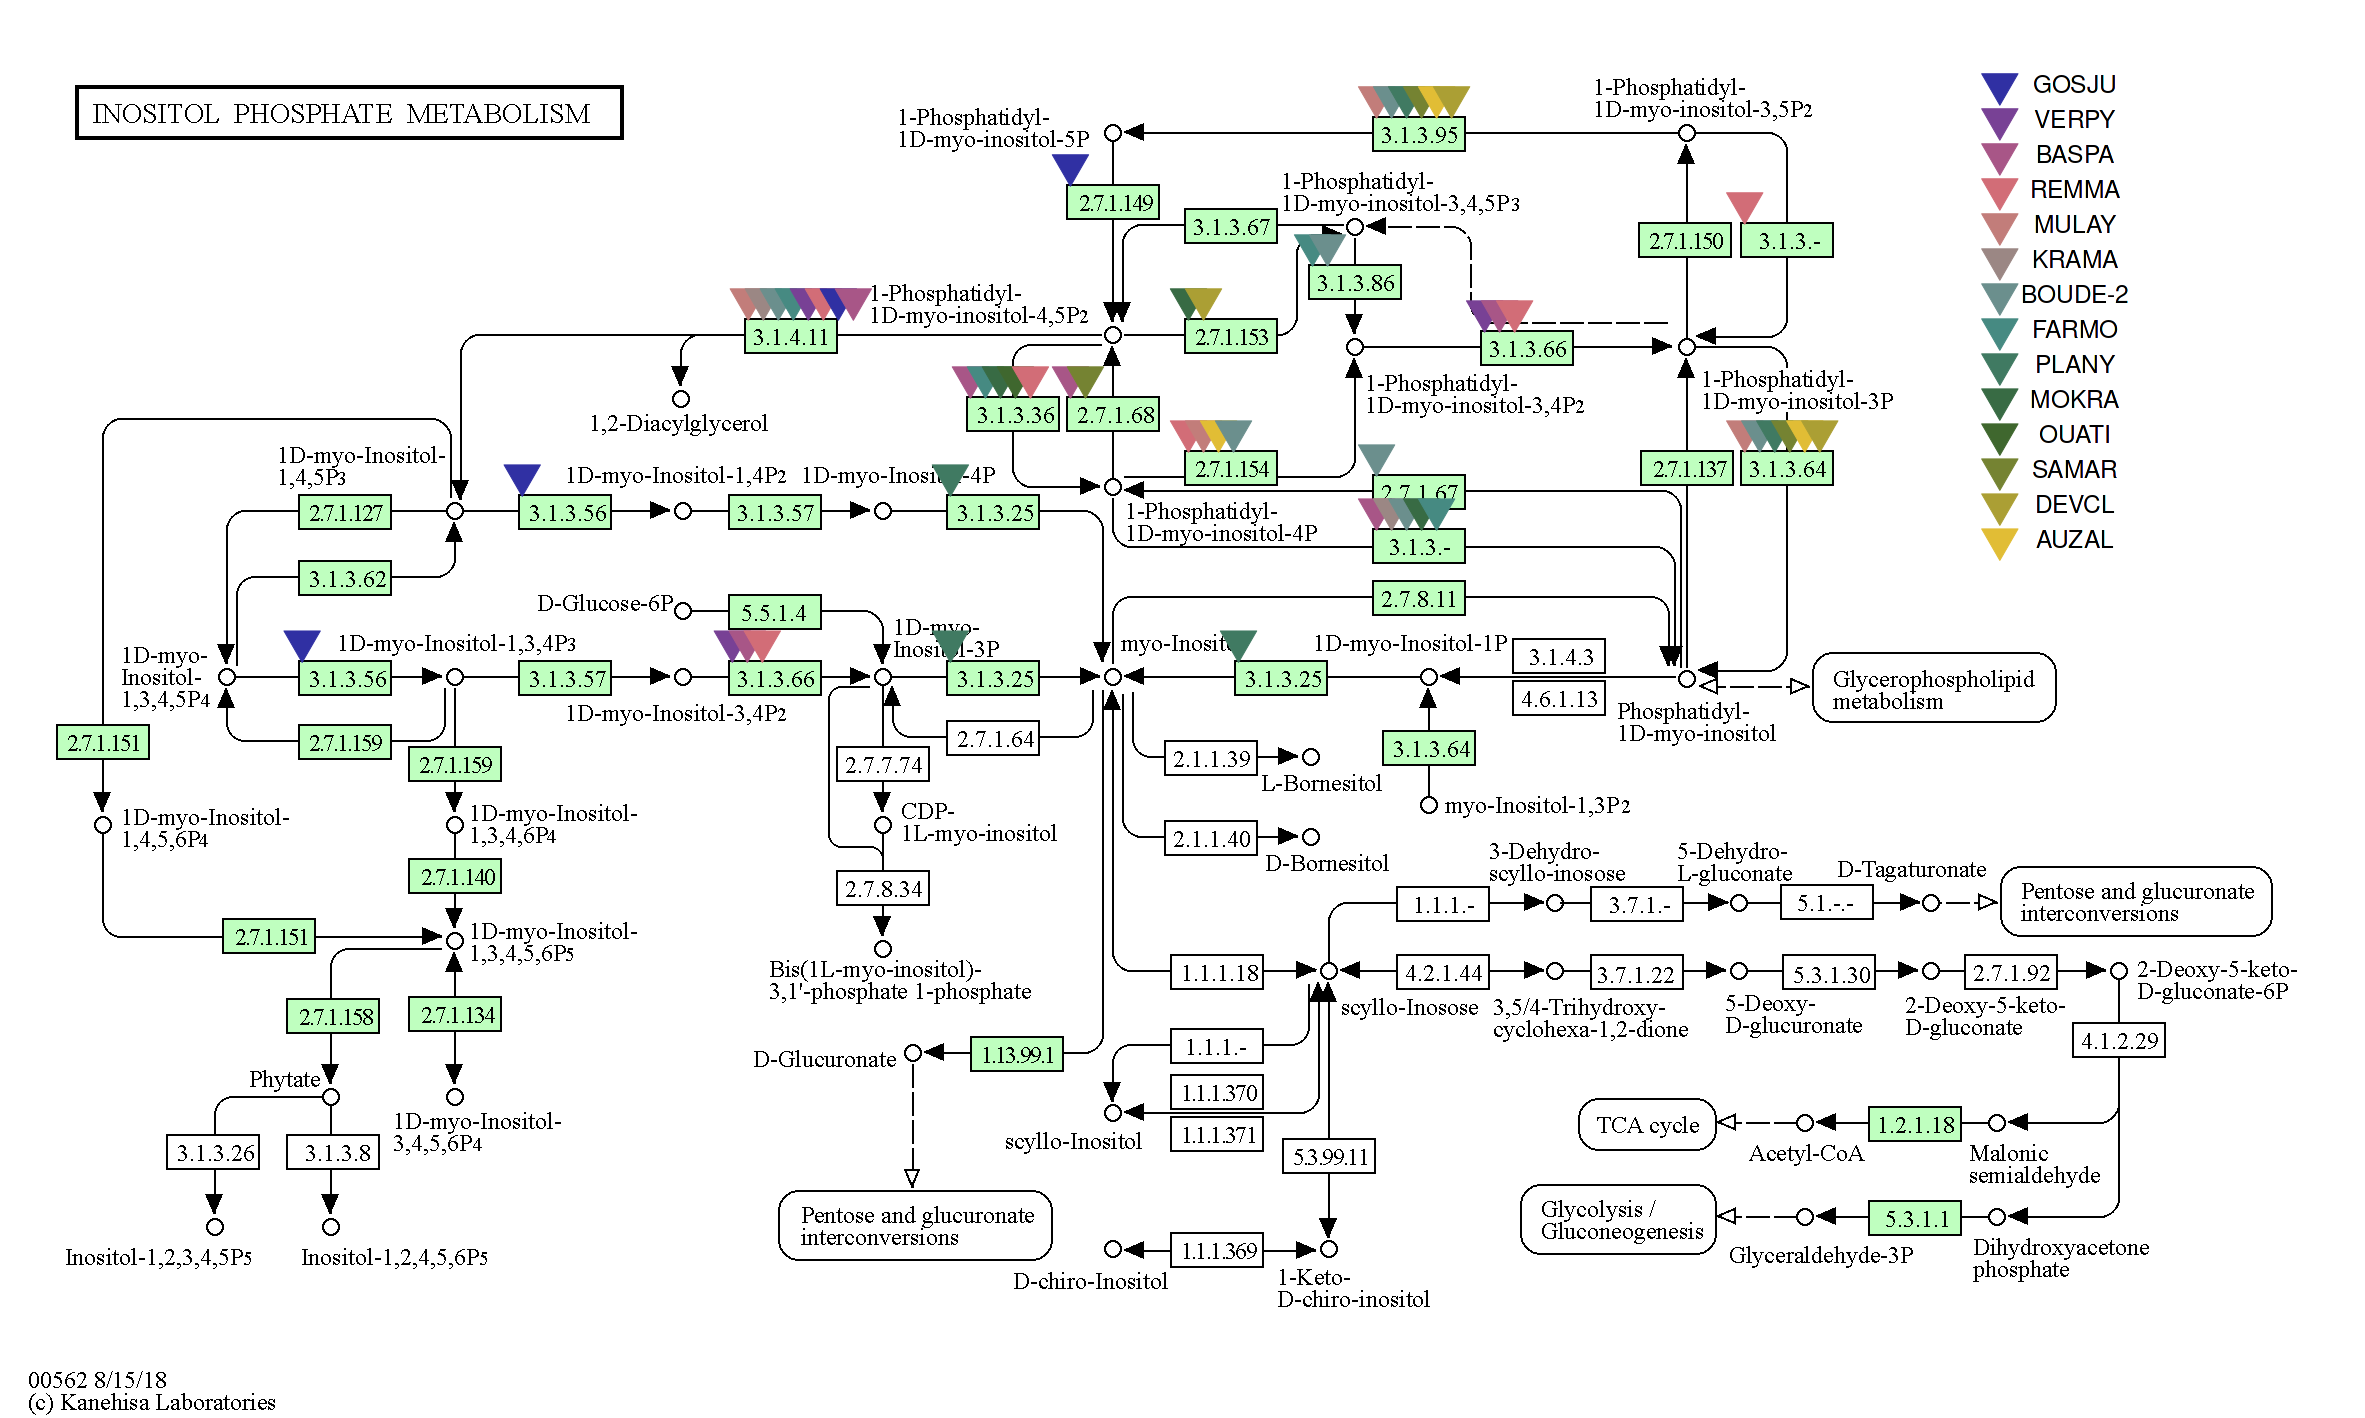
\includegraphics[width=\textwidth]{Images/hsa00562.png}
            \end{figure}
        \end{column}
        \begin{column}{.25\textwidth}
            {\fontsize{3pt}{3.6pt}\selectfont
                \csvreader[
                    tabular = ll,
                    separator = tab,
                    table head = \textbf{Complexes:}\\,
                ]{data/hsa00562.tsv}%
                {ec=\ec,n=\num,name=\name}
                {\ec \\ \name}
            }
        \end{column}
    \end{columns}
\end{frame}

\begin{frame}
    \frametitle{\emoji{compass} Results -- Over-representation analysis -- KEGG -- Choline metabolism in cancer}
    \begin{figure}
        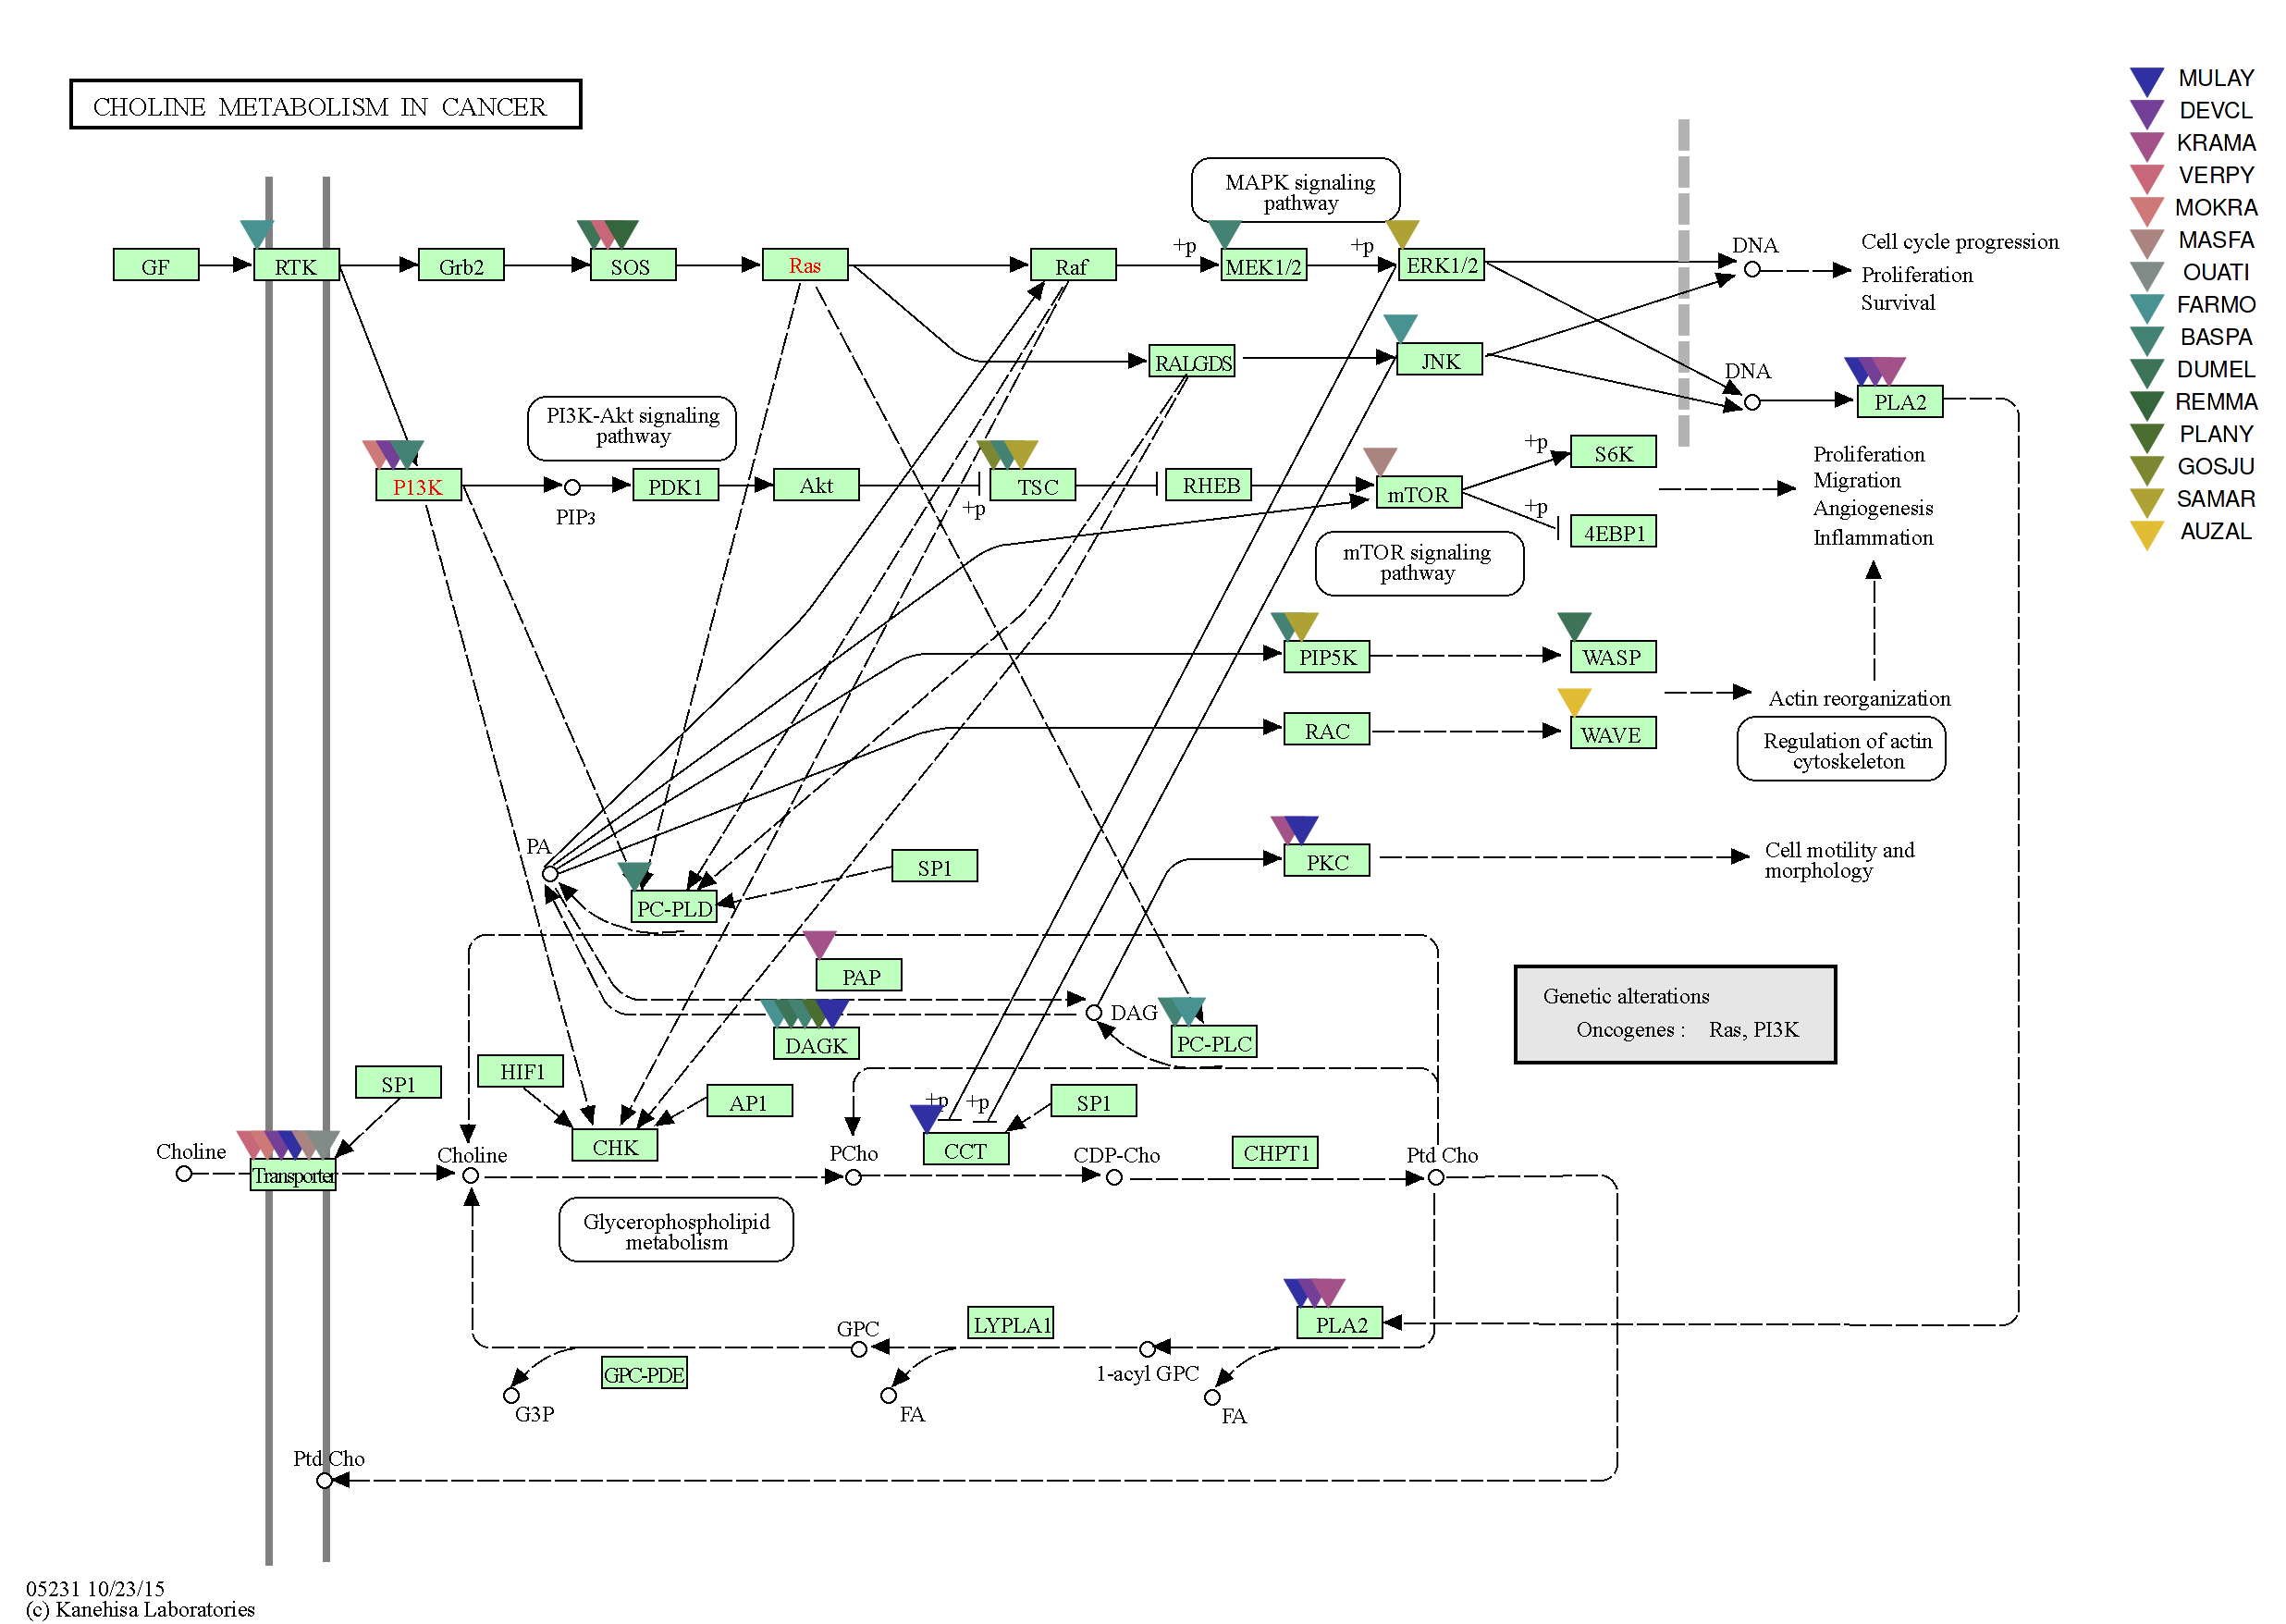
\includegraphics[width=.8\textwidth]{Images/hsa05231.png}
    \end{figure}
\end{frame}

\begin{frame}
    \frametitle{\emoji{monocle-face} Results -- Confirmation panel}
    \begin{figure}
        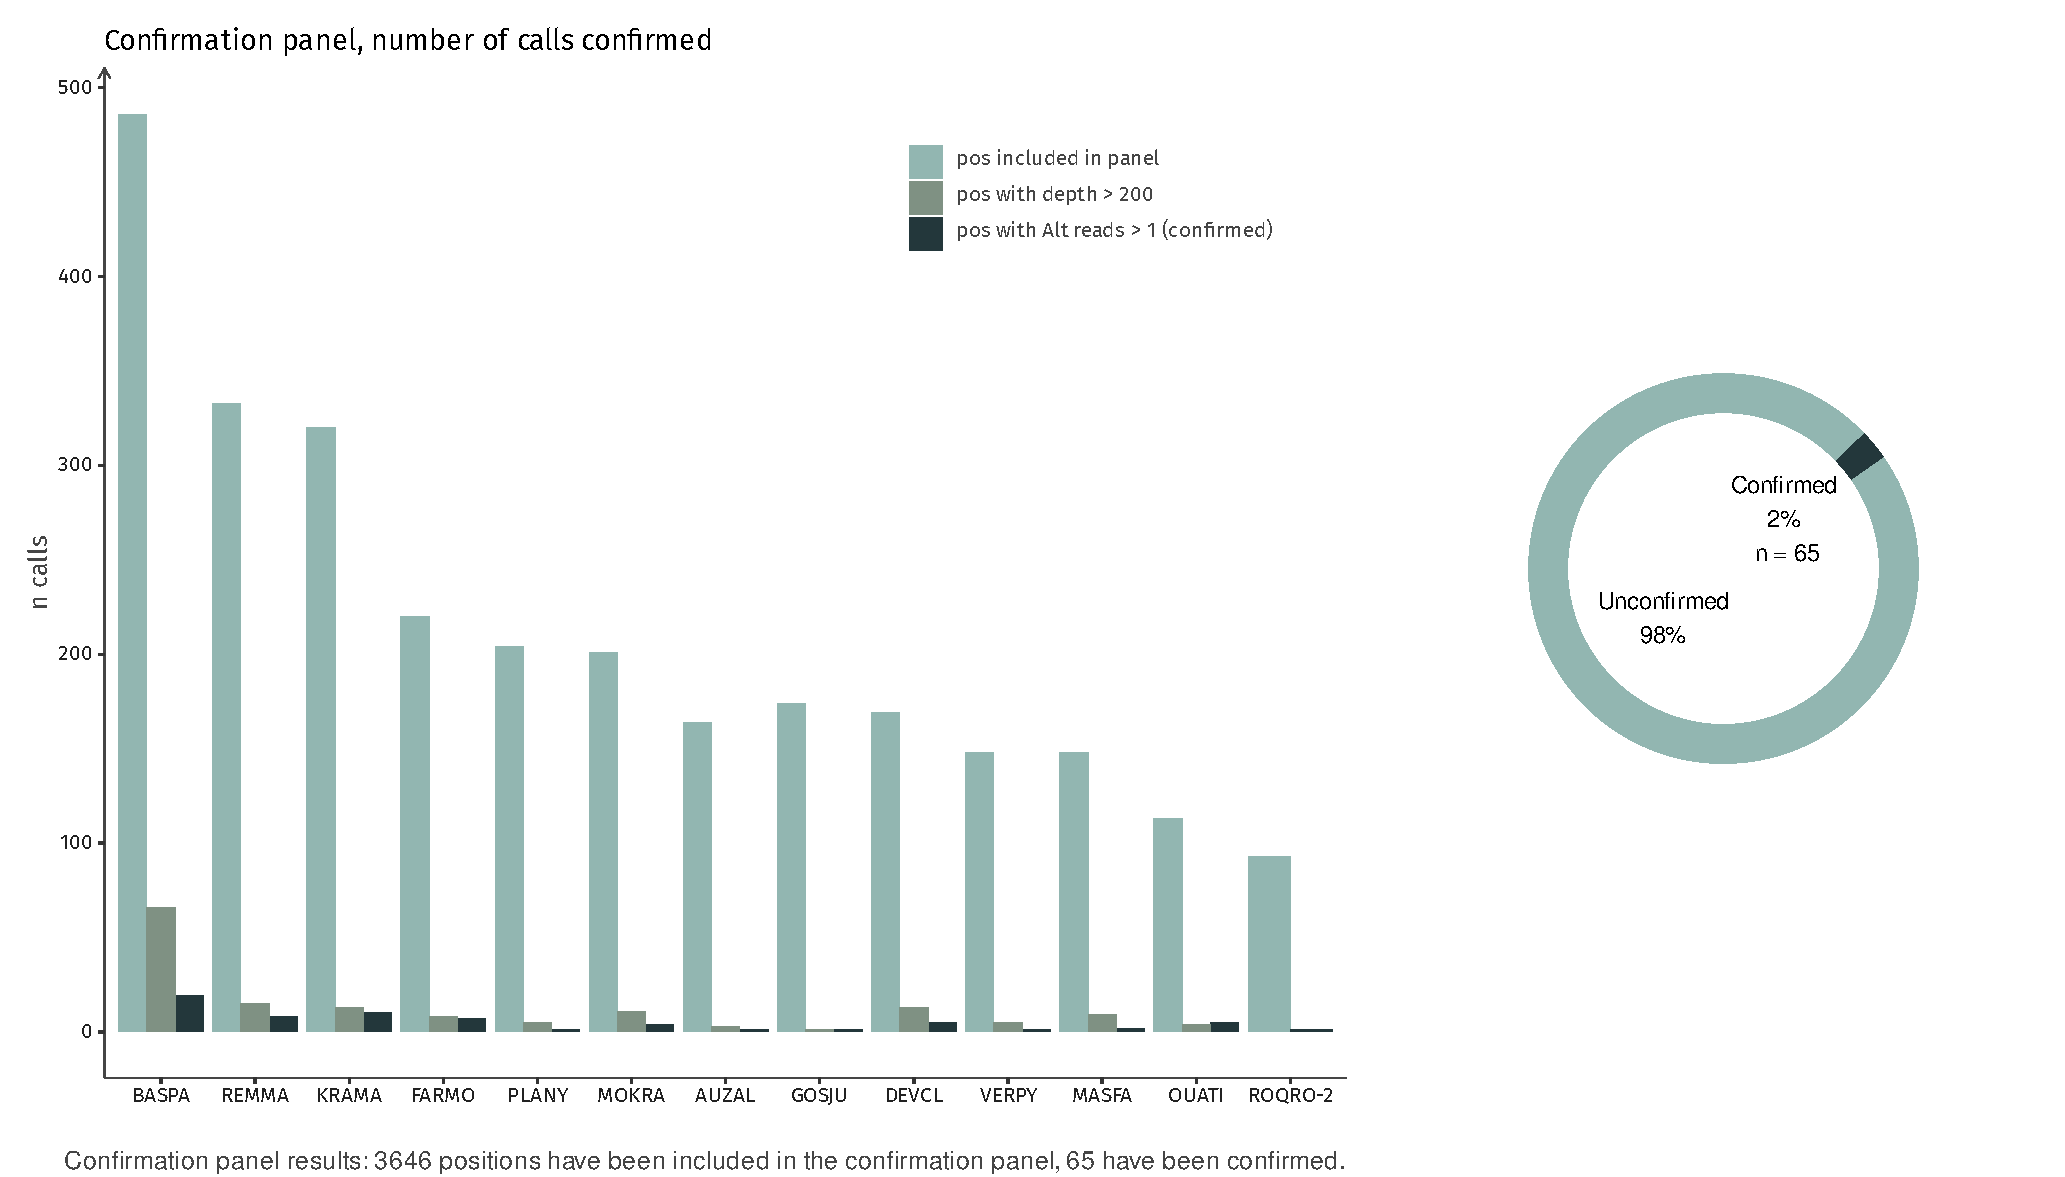
\includegraphics[width=.95  \textwidth]{Images/confirm_1.pdf}
    \end{figure}
\end{frame}

\begin{frame}
    \frametitle{\emoji{monocle-face} Results -- Confirmation panel}
    \begin{figure}
        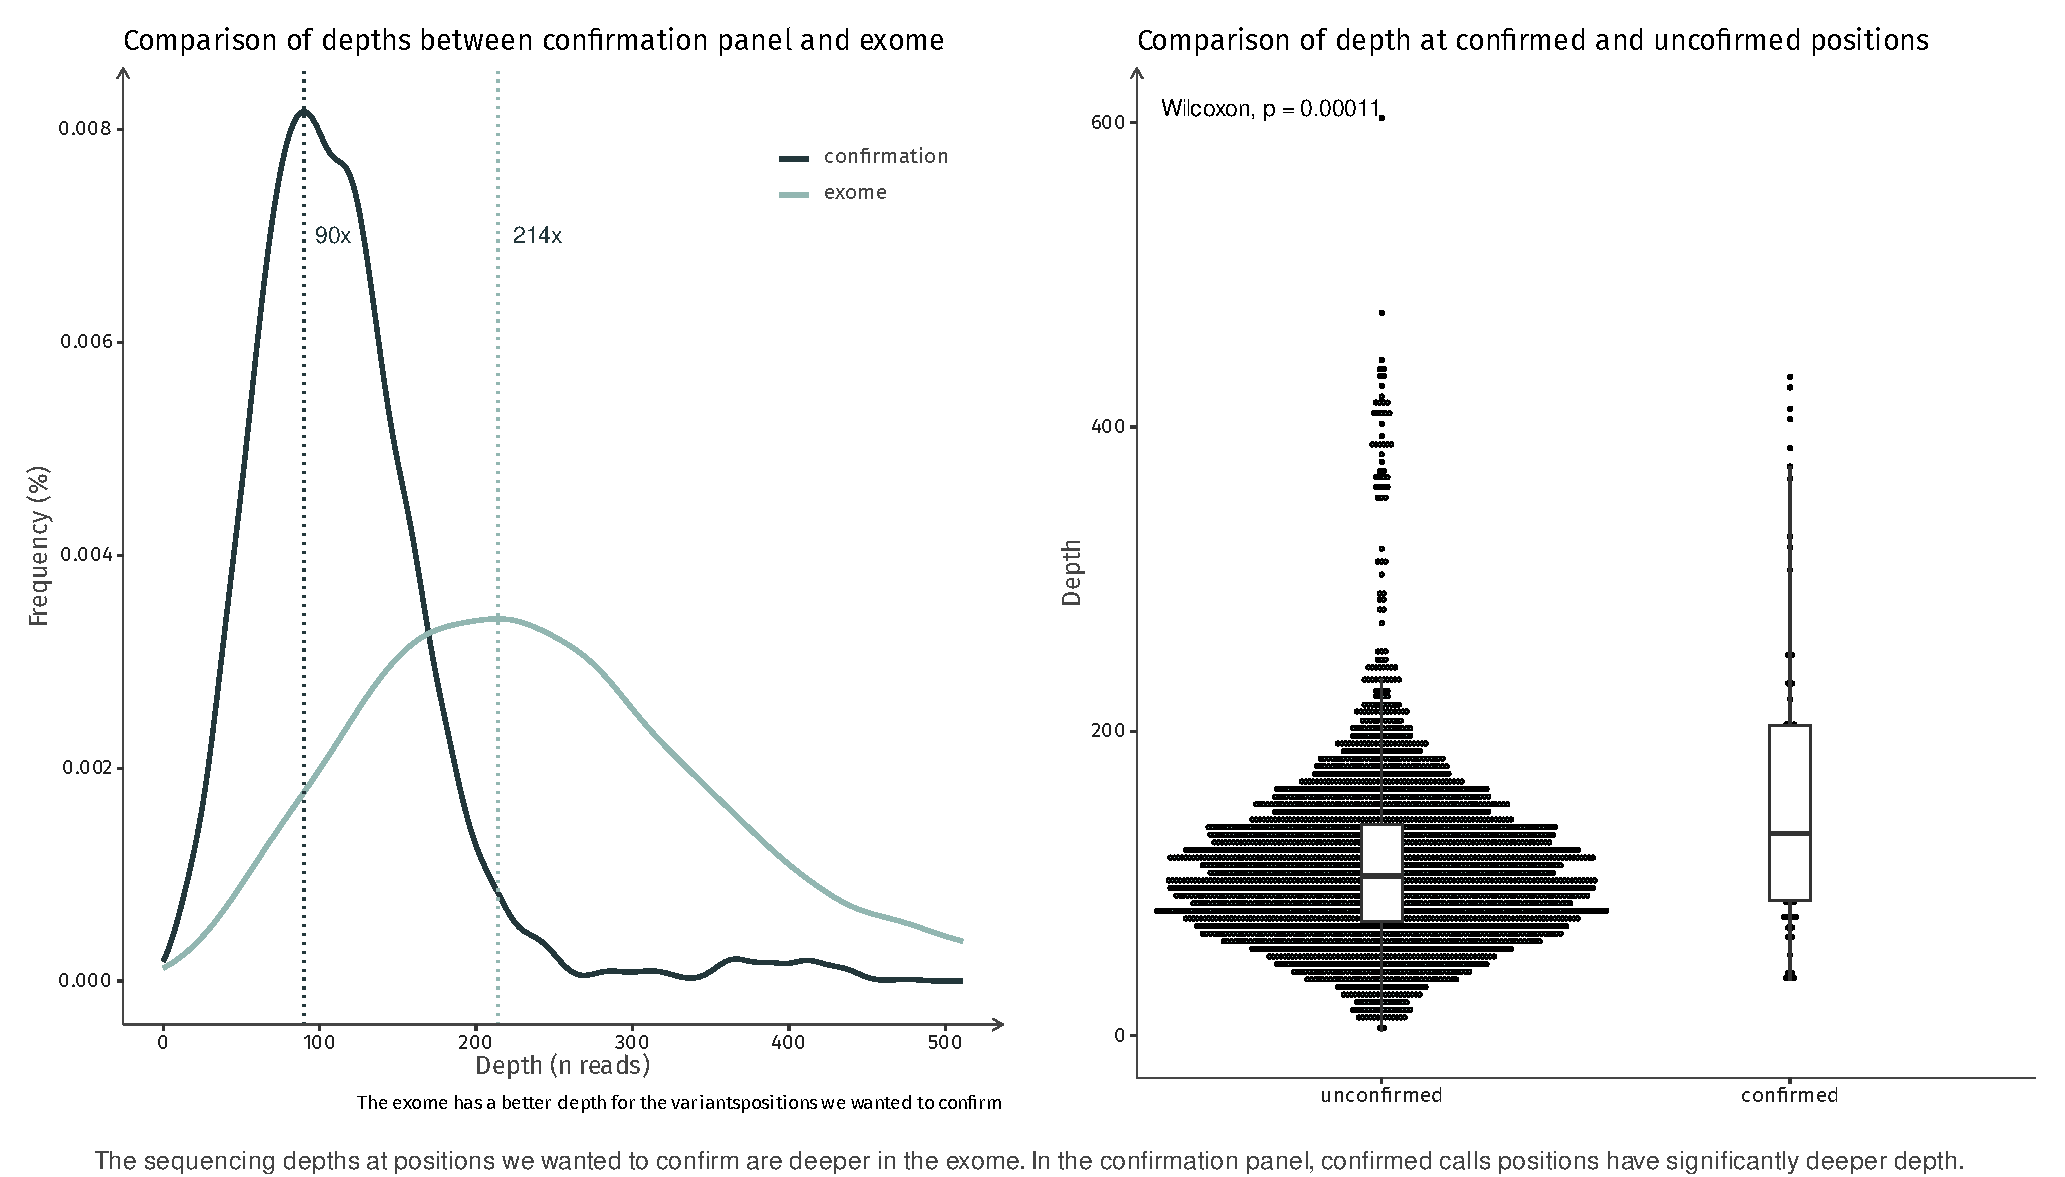
\includegraphics[width=.95  \textwidth]{Images/confirm_2.pdf}
    \end{figure}
\end{frame}

{\setbeamercolor{background canvas}{bg=bgturq}
\begin{frame}[c]
  \metroset{block=fill}
  \vspace{.6cm}
  \begin{alertblock}{\centering \large Conclusions}
    \begin{itemize}
        \item[$\Rrightarrow$] 17 éxomes analysés, environ 300 mutations par cas.
        \item[$\Rrightarrow$] Mutations retrouvées majoritairement à des VAF allant de 1 à 2 \%
        \item[$\Rrightarrow$] Récurrence de mutations sur les gènes connus pour être impliqués dans le cancer: 
        \textit{ALK, ARID1A, KMT2C, NCOA3, NCOR1, NOTCH1, NOTCH2, PIK3CA} et \textit{SMARCA4}.
        \item[$\Rrightarrow$] Net enrichissement de mutations touchant des gènes impliqués dans le métabolisme 
        des Inositol Phosphates.
        \item[$\Rrightarrow$] Panel de confirmation insuffisamment couvert cependant il confirme 65 mutations.
    \end{itemize}
  \end{alertblock}
\end{frame}
}

\begin{frame}[standout]
    Supplementaries
\end{frame}

\begin{frame}
    \frametitle{\emoji{floppy-disk} Methods > Calling > Lancet}
    Source code : \url{https://github.com/nygenome/lancet}
    \vskip 0.2in
    \lstinputlisting[language=bash, caption={lancet -- bash version}, style=mystyle]{Codes/lancet.txt}
\end{frame}

\begin{frame}
    \frametitle{\emoji{floppy-disk} Methods > Calling > Manta puis Strelka}
    \begin{footnotesize}
        Manta : \url{https://github.com/Illumina/manta}
        \lstinputlisting[language=bash, caption={manta -- bash version}, style=mystyle]{Codes/manta.txt}
        Strelka : \url{https://github.com/Illumina/strelka}
        \lstinputlisting[language=bash, caption={strelka -- bash version}, style=mystyle]{Codes/strelka.txt}
    \end{footnotesize}
\end{frame}

\begin{frame}
    \frametitle{\emoji{floppy-disk} Methods > Calling > Mutect2}
    From : \footnotesize \url{https://gatk.broadinstitute.org/hc/en-us/articles/360035531132}
    \lstinputlisting[language=bash, caption={Mutect2 -- seule étape adaptée -- bash version}, style=mystyle]{Codes/mutect2.txt}
\end{frame}

\end{document}